\documentclass[a4paper,12pt]{report}

% --------------------------
% CODIFICA E LINGUA
% --------------------------
\usepackage[utf8]{inputenc}
\usepackage[T1]{fontenc}
\usepackage[english,italian]{babel}
\usepackage{makecell} 

% --------------------------
% PACCHETTI MATEMATICI
% --------------------------
\usepackage{amsmath, amssymb}
\usepackage{algorithm2e}

% --------------------------
% GESTIONE LINK E RIFERIMENTI
% --------------------------
\usepackage{hyperref}
\hypersetup{
    colorlinks=true,
    linkcolor=blue,
    urlcolor=blue,
    pdftitle={Appunti di Reti e Informatica},
    pdfauthor={Luca Argentino},
    pdfpagemode=FullScreen,
}

% --------------------------
% LISTE, BOX, E AMBIENTI
% --------------------------
\usepackage{enumitem}
\usepackage{tcolorbox}
\usepackage{xifthen}
\tcbuselibrary{most}
\usepackage{tikz}

% --------------------------
% GRAFICA E IMMAGINI
% --------------------------
\usepackage{graphicx}
\usepackage{float}
\usepackage{caption}

% --------------------------
% TABELLE
% --------------------------
\usepackage{array}
\usepackage{tabularx}
\usepackage{booktabs}
\usepackage{longtable}
\usepackage{ltablex}
\usepackage{multirow}
\keepXColumns

% --------------------------
% LAYOUT E INTESTAZIONI
% --------------------------
\usepackage[margin=2cm]{geometry}
\usepackage{fancyhdr}
\usepackage{titlesec}

% --------------------------
% COLORI AGGIUNTIVI
% --------------------------
\usepackage{xcolor}
\usepackage{colortbl}

% --------------------------
% FIGURE E LAYOUT TESTO
% --------------------------
\usepackage{subcaption}
\usepackage{wrapfig}

% --------------------------
% TIKZ LIBRERIE
% --------------------------
\usetikzlibrary{arrows.meta, positioning, calc, decorations.pathreplacing, shapes.geometric, shapes.multipart, fit, backgrounds}

% --------------------------
% COLORI UNIBO
% --------------------------
\definecolor{uniboblue}{RGB}{0,68,136}
\definecolor{unibolight}{RGB}{220,235,250}
\definecolor{warnyellow}{RGB}{180,120,0}
\definecolor{warnyellowbg}{RGB}{255,248,225}
\definecolor{slidebg}{RGB}{245,248,255}
\definecolor{alertred}{RGB}{180,0,0}
\definecolor{okgreen}{RGB}{0,120,50}
\definecolor{routerblue}{RGB}{30,80,160}
\definecolor{fabricpurple}{RGB}{100,50,150}

% --------------------------
% IMPOSTAZIONI PERSONALIZZATE
% --------------------------
\renewcommand{\arraystretch}{1.2}
\setlength{\parindent}{0pt}
\setlist[itemize]{noitemsep, topsep=4pt}
\setlist[enumerate]{noitemsep, topsep=4pt}

% =========================================================
\newtcolorbox{defbox}[2][]{%
  colback=green!10,
  colframe=green!65!black,
  title={Definizione\ifstrempty{#2}{}{ -- #2}},
  breakable,
  #1
}

\newtcolorbox{notebox}[2][]{%
  colback=yellow!10,
  colframe=yellow!60!black,
  title={Nota\ifstrempty{#2}{}{ -- #2}},
  breakable,
  #1
}

\newtcolorbox{esempiobox}[2][]{%
  colback=blue!10,
  colframe=blue!65!black,
  title={Esempio\ifstrempty{#2}{}{ -- #2}},
  breakable,
  #1
}

\newtcolorbox{urgentbox}[2][]{%
  colback=red!10,
  colframe=red!75!black,
  title={Importante\ifstrempty{#2}{}{ -- #2}},
  breakable,
  #1
}

\usepackage[many]{tcolorbox}

% Definizione della box per i collegamenti tra capitoli
\newtcolorbox{collegamentobox}[1][]{
  colback=orange!5!white,
  colframe=orange!75!black,
  fonttitle=\bfseries,
  title= Collegamento Inter-Capitolo,
  boxrule=1pt,
  arc=3pt,
  #1
}

\tcbset{
  defbox/.style={colback=unibolight,colframe=uniboblue,fonttitle=\bfseries,breakable,left=6pt,right=6pt},
  alertbox/.style={colback=red!8,colframe=alertred,fonttitle=\bfseries\color{alertred},breakable,left=6pt,right=6pt},
  keybox/.style={colback=green!8,colframe=okgreen,fonttitle=\bfseries\color{okgreen},breakable,left=6pt,right=6pt}
}
% =========================================================

\title{Reti di Calcolatori (Modulo II) \\ Capitolo 5: Livello di Rete -- Piano dei Dati}
\author{Luca Argentino}
\date{2025 -- 2026}

\begin{document}
\maketitle
\tableofcontents
\newpage

\setcounter{chapter}{4}

% ============================================================
\chapter{Livello di Rete: Piano dei Dati (\textit{Data Plane})}
% ============================================================

Il livello di rete (\textit{network layer}) è responsabile del trasporto dei segmenti dal lato mittente al lato destinatario attraverso una rete potenzialmente composta da molti router intermedi. Questo capitolo si concentra sul \textbf{piano dei dati} (\textit{data plane}), ovvero la parte del livello di rete che opera localmente su ogni singolo router e determina come un datagramma in arrivo su una porta di ingresso viene instradato verso la porta di uscita corretta.

% ============================================================
\section{Panoramica del Livello di Rete}
% ============================================================

\subsection{Ruolo del livello di rete}

Il livello di rete opera in ogni host e in ogni router della rete. Le sue responsabilità principali sono:

\begin{itemize}
    \item \textbf{Lato mittente}: incapsulare i segmenti provenienti dal livello di trasporto in \textit{datagrammi}.
    \item \textbf{Lato destinatario}: consegnare i segmenti al livello di trasporto, estraendoli dai datagrammi ricevuti.
    \item \textbf{Nei router}: esaminare i campi dell'header di tutti i datagrammi IP che li attraversano e decidere verso quale porta di uscita inoltrarli.
\end{itemize}

\begin{figure}[H]
    \centering
    \begin{tikzpicture}[
        node distance=0.8cm and 1.5cm,
        layer/.style={rectangle, draw, fill=blue!15, minimum width=2.2cm, minimum height=0.55cm, font=\small},
        netlayer/.style={rectangle, draw, fill=red!20, minimum width=2.2cm, minimum height=0.55cm, font=\small\bfseries},
        router/.style={rectangle, draw, fill=orange!20, minimum width=2.2cm, minimum height=0.55cm, font=\small},
    ]
    % Host A (sinistra)
    \node[layer] (appA) {applicazione};
    \node[layer, below=of appA] (trA) {trasporto};
    \node[netlayer, below=of trA] (netA) {rete};
    \node[layer, below=of netA] (dlA) {data link};
    \node[layer, below=of dlA] (phyA) {fisico};
    \node[above=0.2cm of appA, font=\bfseries\small] {Host A};

    % Router 1
    \node[router, right=2cm of netA] (net1) {rete};
    \node[router, below=of net1] (dl1) {data link};
    \node[router, below=of dl1] (phy1) {fisico};
    \node[above=0.2cm of net1, font=\bfseries\small] {Router 1};

    % Router 2
    \node[router, right=2cm of net1] (net2) {rete};
    \node[router, below=of net2] (dl2) {data link};
    \node[router, below=of dl2] (phy2) {fisico};
    \node[above=0.2cm of net2, font=\bfseries\small] {Router 2};

    % Host B (destra)
    \node[layer, right=2cm of net2] (netB) {rete};
    \node[layer, above=of netB] (trB) {trasporto};
    \node[layer, above=of trB] (appB) {applicazione};
    \node[layer, below=of netB] (dlB) {data link};
    \node[layer, below=of dlB] (phyB) {fisico};
    \node[above=0.2cm of appB, font=\bfseries\small] {Host B};

    % Frecce di collegamento
    \draw[->, thick, uniboblue] (phyA) -- (phy1);
    \draw[->, thick, uniboblue] (phy1) -- (phy2);
    \draw[->, thick, uniboblue] (phy2) -- (phyB);

    % Evidenzia il livello rete
    \node[draw=red!80, dashed, thick, fit=(netA)(net1)(net2)(netB),
          inner sep=6pt] {};
    \end{tikzpicture}
    \caption{Il livello di rete è presente in ogni host e in ogni router. I router intermedi gestiscono solo i livelli inferiori (fino al livello di rete).}
    \label{fig:network-layer-stack}
\end{figure}

\subsection{Le due funzioni chiave del livello di rete}

\begin{defbox}{Forwarding vs Routing}
Il livello di rete svolge due funzioni fondamentali e distinte:
\begin{itemize}
    \item \textbf{Forwarding\footnote{Vedi anche  sezione 3.3.7 capitolo 3} (Inoltro)}: sposta i pacchetti dall'ingresso all'uscita appropriata di un \textit{singolo} router (ovvero a quale interfaccia inoltrare un pacchetto in base alla destinazione). È un'operazione \textit{locale}, rapida, eseguita in hardware nel piano dei dati.
    \item \textbf{Routing\footnote{Vedi anche sezione 3.3.8 capitolo 3} (Instradamento)}: determina il percorso (\textit{path}) che i pacchetti devono seguire dalla sorgente alla destinazione attraverso l'intera rete. È un'operazione \textit{globale}, più lenta, eseguita in software nel piano di controllo (che vedremo nel dettsglio nel capitolo 6).
\end{itemize}
\end{defbox}

\begin{esempiobox}{Analogia con un viaggio in auto}
\begin{itemize}
    \item Il \textbf{forwarding} è come attraversare un singolo svincolo autostradale: sei già lì e devi solo scegliere la rampa giusta in base alla tua destinazione. E' quindi l'azione pratica
    \item Il \textbf{routing} è come pianificare l'intero viaggio da Bologna a Londra: decidi in anticipo quale autostrada prendere, dove cambiare direzione, ecc. E' quiindi una decisione logica
\end{itemize}
\end{esempiobox}

Il forwarding si basa su una \textbf{forwarding table} (tabella di inoltro): il router legge un valore dall'header del pacchetto in arrivo e lo usa come indice in questa tabella per determinare la porta di uscita corretta.



\newpage
\subsection{Piano dei dati e piano di controllo }
\label{:piano controllo}
\begin{defbox}{Data Plane e Control Plane}
\begin{itemize}
    \item \textbf{Piano dei dati (\textit{Data Plane})}: funzione \textit{locale} per ogni router. Determina come un datagramma in arrivo su una porta di ingresso viene inoltrato a una porta di uscita. Viene utilizzata per il forwarding .Opera in \textbf{nanosecondi} (hardware).
    \item \textbf{Piano di controllo (\textit{Control Plane})}: logica a livello di \textit{rete intera}. Determina come i datagrammi vengono instradati lungo i router dal sorgente alla destinazione. Opera in \textbf{millisecondi} (software).
\end{itemize}
\end{defbox}

Esistono due approcci per il piano di controllo:

\begin{enumerate}
    \item \textbf{Algoritmi di routing tradizionali}: implementati nei router stessi. Ogni router esegue un algoritmo di routing e i router si scambiano informazioni tra di loro per costruire le tabelle di forwarding.
    \item \textbf{Software-Defined Networking (SDN)}: un controller remoto (logicamente centralizzato) calcola e distribuisce le tabelle di forwarding a tutti i router. I router si limitano a eseguire le istruzioni del controller.
\end{enumerate}




\newpage
% ============================================================
\subsection*{Piano di controllo: I due approcci a confronto}
% ============================================================

Il \textbf{piano di controllo} (\textit{control plane}) 
Esistono due filosofie architetturali radicalmente diverse per implementarlo.

% ------- IMMAGINE 1 -----------------------------------------
\subsection*{1) Piano di controllo per-router}

\begin{figure}[H]
    \centering
    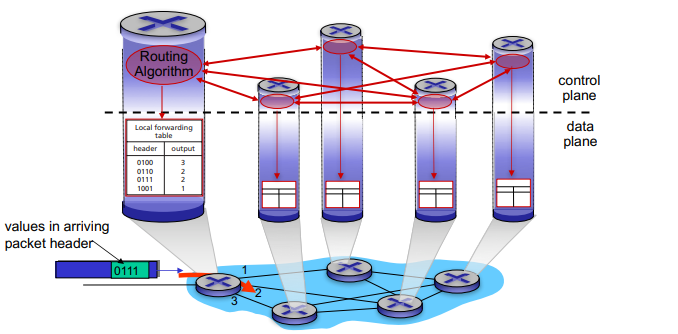
\includegraphics[width=0.82\textwidth]{router_1}
    \caption{Approccio 1 -- Piano di controllo per-router (\textit{per-router control plane}).}
    \label{fig:per_router_cp}
\end{figure}

Come illustrato nella Figura \ref{fig:per_router_cp}, in questo approccio ogni router fisico (rappresentato dal cilindro blu) è indipendente e suddiviso in due componenti separati dalla linea tratteggiata orizzontale. Il sistema si articola nei seguenti punti:

\begin{enumerate}
    \item \textbf{Control plane} (sopra la linea tratteggiata): è rappresentato dal cerchio rosso (``Routing Algorithm''), che indica un processo software in esecuzione in background (es.\ un demone di sistema come \texttt{ospfd}).
    \item \textbf{Data plane} (sotto la linea tratteggiata): ospita la \textbf{local forwarding table}, la tabella prodotta dal demone di routing locale e utilizzata direttamente dall'hardware per instradare i pacchetti.
    \item \textbf{Scambio di messaggi}: le \textbf{frecce rosse} che collegano i cerchi rappresentano i messaggi del protocollo di routing scambiati tra i demoni dei vari router per condividere informazioni sulla rete (come annunci di topologia, costi dei link, ecc.).
    \item \textbf{Operazione di forwarding}: nella parte inferiore dello schema è mostrato l'arrivo di un pacchetto (es.\ con valore \texttt{0111} nell'header). Il valore viene confrontato con la forwarding table: l'entry corrispondente (\texttt{0111 $\to$ 2}) fa sì che il pacchetto venga fisicamente commutato verso la porta 2 (movimento indicato dalla freccia rosso chiaro).
\end{enumerate}

\newpage
\subsubsection*{Come funziona il piano di controllo per-router}

Nell'approccio tradizionale il controllo è \textbf{completamente distribuito}:
non esiste alcun coordinatore centrale. Ogni router esegue autonomamente il
proprio demone di routing, che:

\begin{enumerate}
    \item \textbf{Scopre i vicini}: tramite messaggi \textit{hello} inviati
          sulle interfacce dirette, il router apprende quali altri router
          sono raggiungibili direttamente e a che costo.
    \item \textbf{Scambia informazioni di topologia}: le frecce rosse in
          figura rappresentano i messaggi di protocollo (LSA in OSPF,
          distance vectors in RIP, UPDATE in BGP) che i demoni si
          inviano reciprocamente attraverso la rete fisica.
    \item \textbf{Esegue l'algoritmo di routing}: sulla base delle
          informazioni raccolte, ogni demone calcola autonomamente i
          percorsi minimi (es.\ Dijkstra per OSPF, Bellman-Ford per RIP).
    \item \textbf{Scrive la forwarding table}: il risultato del calcolo
          viene scritto nella tabella locale del data plane, usata poi
          dall'hardware di switching in nanosecondi.
\end{enumerate}

\begin{notebox}{Proprietà emergente del sistema distribuito}
La visione globale della rete \textbf{non esiste esplicitamente} in nessun
posto: emerge dall'interazione collettiva di tutti i demoni. Questa
proprietà conferisce alla rete una robustezza intrinseca -- se un router
si guasta, gli altri rilevano l'evento (link down, timeout hello) e
\textbf{riconvergono autonomamente} calcolando nuovi percorsi, senza
bisogno di un coordinatore che intervenga.
\end{notebox}

\newpage
% ------- IMMAGINE 2 -----------------------------------------
\subsection*{2) SDN}

\begin{figure}[H]
    \centering
    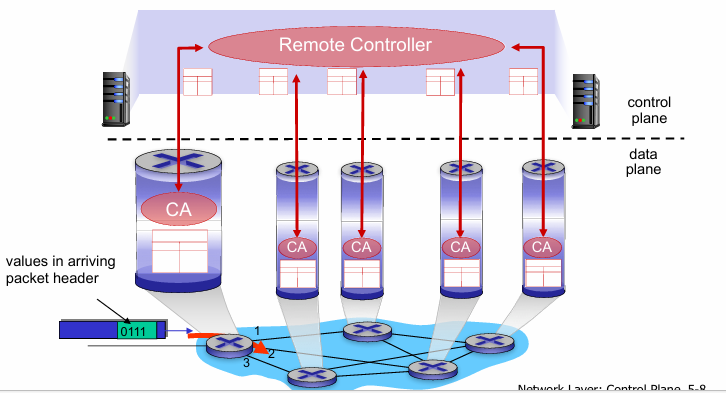
\includegraphics[width=0.82\textwidth]{router_2}
    \caption{Approccio 2 -- Piano di controllo logicamente centralizzato (\textit{SDN: Software-Defined Networking}).}
    \label{fig:sdn_cp}
\end{figure}

Come illustrato nella Figura \ref{fig:sdn_cp}, questo approccio separa fisicamente l'intelligenza della rete dai dispositivi di inoltro. Il funzionamento si basa sui seguenti elementi chiave:

\begin{enumerate}
    \item \textbf{Remote Controller:} rappresentato dall'ellisse rosa in alto (nel cloud del control plane), è un'entità software tipicamente eseguita su server remoti, quindi fisicamente separata dai router.
    \item \textbf{Control Agent (CA):} i router fisici non elaborano più alcun algoritmo di routing in autonomia. Al loro interno, il cerchio etichettato \textbf{CA} indica un agente software minimale il cui unico compito è \emph{comunicare con il controller remoto} (tramite le frecce rosse bidirezionali) e \emph{applicare le istruzioni ricevute} scrivendole nella forwarding table locale.
    \item \textbf{Data plane e Forwarding:} posizionato sotto la linea tratteggiata, il data plane continua a funzionare esattamente come nell'approccio tradizionale. Ad esempio, il valore \texttt{0111} letto nell'header di un pacchetto in ingresso viene cercato nella tabella di inoltro per commutare l'unità dati verso la porta di uscita corretta.
\end{enumerate}

\subsubsection*{Come funziona il piano di controllo SDN}

Nell'approccio SDN il controllo è \textbf{logicamente centralizzato}:

\begin{enumerate}
    \item \textbf{I CA raccolgono informazioni}: ogni Control Agent informa
          il Remote Controller sullo stato locale -- porte attive, costi
          dei link, statistiche di traffico.
    \item \textbf{Il controller ha la visione globale}: raccogliendo i dati
          di tutti i CA, il controller mantiene una \textit{network view}
          completa e aggiornata dell'intera topologia, cosa impossibile in
          un singolo router nell'approccio distribuito.
    \item \textbf{Il controller calcola le forwarding table}: eseguendo
          algoritmi di routing (o policy arbitrariamente complesse) su
          questa visione globale, il controller calcola la forwarding
          table ottima per \emph{ciascun} router.
    \item \textbf{Il controller distribuisce le tabelle}: tramite il
          protocollo OpenFlow (o simili), le tabelle vengono inviate ai CA
          dei rispettivi router, che le installano nel data plane locale.
    \item \textbf{Il data plane esegue autonomamente}: una volta installata
          la tabella, il forwarding dei pacchetti avviene in hardware,
          esattamente come nel caso per-router, senza coinvolgere il
          controller per ogni singolo pacchetto.
\end{enumerate}

\begin{notebox}{``Logicamente'' centralizzato}
Il controller è \textbf{logicamente} centralizzato, ma non necessariamente
\textbf{fisicamente} centralizzato. Nella pratica i sistemi SDN moderni
(es.\ ONOS, OpenDaylight) usano controller \textit{replicati} e
distribuiti geograficamente per garantire fault tolerance e scalabilità,
pur presentando all'esterno una vista unica e coerente della rete.
\end{notebox}

% ------- CONFRONTO SINOTTICO --------------------------------
\subsubsection*{Confronto diretto tra i due approcci}

\begin{table}[H]
\centering
\label{tab:cp_comparison}
\begin{tabularx}{\textwidth}{lXX}
\toprule
\textbf{Aspetto}
    & \textbf{Per-router (tradizionale)}
    & \textbf{SDN (logicamente centralizzato)} \\
\midrule
\textbf{Dove gira la logica}
    & Demone di routing su \emph{ogni} router
    & Remote Controller su server separati \\
\addlinespace
\textbf{Visione della rete}
    & Parziale: ogni router vede solo i vicini
    & Globale: il controller vede tutta la topologia \\
\addlinespace
\textbf{Comunicazione tra nodi}
    & I router si parlano direttamente (frecce rosse tra demoni)
    & I CA parlano solo con il controller (frecce rosse verticali) \\
\addlinespace
\textbf{Calcolo dei percorsi}
    & Distribuito su tutti i router, emerge per convergenza
    & Centralizzato nel controller, poi distribuito ai router \\
\addlinespace
\textbf{Flessibilità delle policy}
    & Limitata ai protocolli standard (OSPF, BGP\ldots)
    & Arbitraria: il controller può applicare qualsiasi logica \\
\addlinespace
\textbf{Robustezza}
    & Alta: nessun single point of failure
    & Il controller è un potenziale SPOF (mitigato da repliche) \\
\addlinespace
\textbf{Data plane}
    & Identico nei due casi: forwarding table $\to$ hardware  \\
\addlinespace
\textbf{Velocità di convergenza}
    & Dipende dal protocollo (secondi--minuti)
    & Può essere più rapida con visione globale \\
\addlinespace
\textbf{Esempi reali}
    & Router ISP con OSPF/BGP/RIP
    & Data center (VMware NSX), WAN (Google B4) \\
\bottomrule
\end{tabularx}
\end{table}

\begin{urgentbox}{La distinzione data plane / control plane è invariante}
Un aspetto cruciale da notare guardando entrambe le figure: la
\textbf{linea tratteggiata} che separa control plane e data plane è
presente in \emph{entrambi} gli approcci, e il data plane funziona in modo
identico. La differenza riguarda esclusivamente \emph{dove e come} viene
calcolata la forwarding table -- non il modo in cui essa viene poi usata
per instradare i pacchetti. In entrambi i casi il pacchetto con
\texttt{0111} nell'header viene commutato verso la porta~2 dalla stessa
logica hardware, in nanosecondi.
\end{urgentbox}


\newpage
\subsection{Modello di servizio del livello di rete}

Il \textbf{modello di servizio} definisce le garanzie offerte dal livello di rete ai livelli superiori per il trasporto di datagrammi. Esempi di servizi possibili:

\textit{Per singoli datagrammi}:
\begin{itemize}
    \item Consegna garantita
    \item Consegna garantita con ritardo $< 40$ ms
\end{itemize}

\textit{Per flussi di datagrammi}:
\begin{itemize}
    \item Consegna in ordine
    \item Banda minima garantita
    \item Vincoli sul \textit{jitter} (variazione del ritardo)
\end{itemize}

\begin{table}[H]
\centering
\caption{Modelli di servizio del livello di rete per diverse architetture.}
\label{tab:service-models}
\begin{tabular}{lllllll}
\toprule
\textbf{Architettura} & \textbf{Modello} & \textbf{Banda} & \textbf{Perdita} & \textbf{Ordine} & \textbf{Timing} & \textbf{Congestione} \\
\midrule
Internet & Best effort & Nessuna & No & No & No & No (infer.) \\
ATM & CBR & Costante & Sì & Sì & Sì & No congestion \\
ATM & VBR & Garantita & Sì & Sì & Sì & No congestion \\
ATM & ABR & Min. garant. & No & Sì & No & Sì \\
ATM & UBR & Nessuna & No & Sì & No & No \\
\bottomrule
\end{tabular}
\end{table}

\begin{urgentbox}{Il modello ``Best Effort'' di Internet}
Internet utilizza il modello \textbf{best effort}: nessuna garanzia di consegna, nessuna garanzia sull'ordine, nessun limite sul ritardo. Questo approccio, apparentemente limitante, ha in realtà contribuito al successo di Internet: la semplicità del livello di rete ha permesso di fare girare Internet su qualsiasi tecnologia fisica e ha spinto la complessità ai livelli superiori (TCP per affidabilità, applicazioni per QoS).
\end{urgentbox}



\newpage
% ============================================================
\section{Architettura interna di un Router }
% ============================================================

Un router è un sistema hardware/software complesso il cui compito principale
è ricevere datagrammi sulle porte di ingresso e inoltrarli alle porte di
uscita corrette nel minor tempo possibile.

\vspace{0.5cm}
Comprendere la sua architettura
interna è fondamentale per capire perché il livello di rete si suddivide in
\textit{data plane} e \textit{control plane}, e quali sono i limiti pratici
di prestazione di una rete reale.

% ============================================================
\subsection{Visione architetturale ad alto livello}
% ============================================================

\begin{figure}[H]
    \centering
    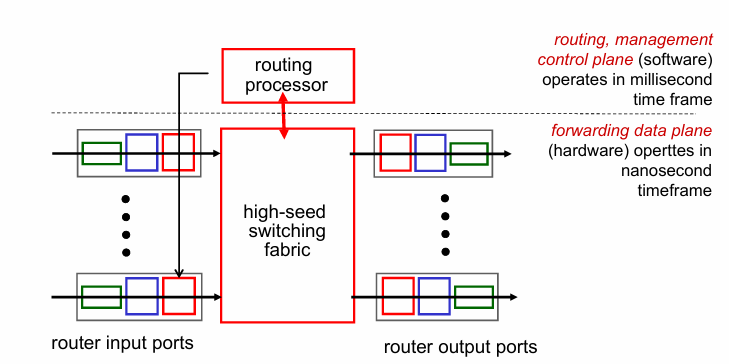
\includegraphics[width=0.82\textwidth]{router_3.png}
    \caption{Architettura ad alto livello di un router generico.}
    \label{fig:router_arch_overview}
\end{figure}

L'architettura interna mostrata nella Figura \ref{fig:router_arch_overview} si articola in quattro componenti fondamentali:

\begin{enumerate}
    \item \textbf{Porte di ingresso:} si occupano della terminazione del collegamento fisico, della decodifica del frame data-link e della ricerca della porta di uscita corretta per ogni datagramma in arrivo.
    \item \textbf{Switching fabric:} costituisce il cuore del router, collegando fisicamente le porte di ingresso alle porte di uscita per il trasferimento dei pacchetti.
    \item \textbf{Porte di uscita:} gestiscono le code di datagrammi in attesa e ne effettuano la trasmissione seriale sul link fisico uscente.
    \item \textbf{Routing processor:} esegue le funzioni di controllo (control plane), tra cui l'elaborazione dei protocolli di routing e la gestione delle tabelle di inoltro.
\end{enumerate}

Come evidenziato dalla linea tratteggiata, la struttura separa nettamente il \textbf{data plane}, operante in hardware su scale temporali di nanosecondi, dal \textbf{control plane}, gestito via software con tempi di reazione nell'ordine dei millisecondi.
La distinzione temporale è fondamentale:

\begin{itemize}
    \item Il \textbf{routing processor} (control plane) aggiorna le tabelle
          di forwarding in risposta a cambiamenti di topologia: questi
          eventi accadono raramente e si misurano in \textbf{millisecondi}.
    \item Le \textbf{porte di ingresso} e lo \textbf{switching fabric} (data
          plane) devono processare ogni singolo pacchetto: a 100~Gbps
          arriva un pacchetto ogni pochi \textbf{nanosecondi}, quindi
          l'intera logica di forwarding deve essere implementata in
          hardware, non in software.
\end{itemize}

\newpage
\begin{urgentbox}{Obiettivo di progetto: line-rate forwarding}
Il vincolo fondamentale di ogni router ad alte prestazioni è operare alla
\textbf{velocità del link} (\textit{line rate}): se un link opera a $R$~bps
e i pacchetti hanno dimensione media $L$~bit, arriva un nuovo pacchetto ogni
$L/R$ secondi. Tutto il processo di ricezione, lookup nella forwarding table
e commutazione deve completarsi entro questo intervallo, altrimenti si
formano code e si perdono pacchetti. Questo giustifica la replica della
forwarding table in ogni porta di ingresso e il suo mantenimento in TCAM\footnote{Ternary-Content-Adressable-Memory: Si tratta di un tipo speciale di memoria ad alta velocità utilizzata nei dispositivi di rete ad alte prestazioni (router e switch di livello 3) per velocizzare le operazioni di ricerca e inoltro dei pacchetti}.
\end{urgentbox}

% ============================================================
\subsection{Porte di ingresso (\textit{Input Ports})}
% ============================================================

Ogni porta di ingresso è un mini-sistema su tre livelli che opera in
pipeline:

\begin{figure}[H]
    \centering
    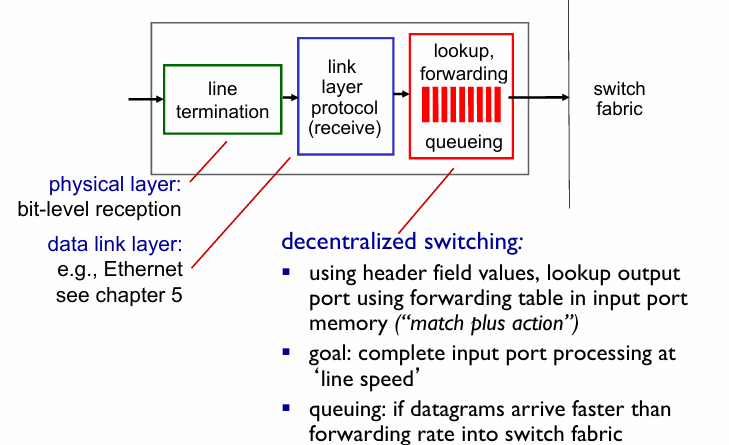
\includegraphics[width=0.88\textwidth]{router_4.png}
    \caption{Struttura interna di una porta di ingresso.}
    \label{fig:input_port_functions}
\end{figure}

Come illustrato nella Figura \ref{fig:input_port_functions}, l'elaborazione all'interno di una porta di ingresso avviene attraverso tre stadi in cascata, da sinistra a destra:

\begin{enumerate}
    \item \textbf{Line termination} (riquadro verde): si occupa della ricezione fisica bit-a-bit dal link, svolgendo le funzioni tipiche del \textit{livello fisico}.
    \item \textbf{Link layer protocol} (riquadro blu): elabora il protocollo data-link (es.\ Ethernet) decodificando il frame, rimuovendone l'header ed estraendo il datagramma IP. Questo stadio corrisponde al \textit{livello data link}.
    \item \textbf{Lookup, forwarding e queueing} (riquadro rosso): costituisce il nucleo operativo del data plane. In questa fase vengono letti i campi dell'header IP e viene consultata la \textbf{forwarding table locale} per determinare la corretta porta di uscita. Se lo switch fabric risulta occupato, il datagramma viene temporaneamente messo in coda.
\end{enumerate}

L'output di questo terzo e ultimo stadio andrà poi ad alimentare direttamente lo \textit{switch fabric}.

\newpage
\subsection{Switching decentralizzato e intro agli algoritmi di lookup}

Il termine \textbf{decentralized switching} indica che la decisione di
forwarding avviene \emph{localmente nella porta di ingresso}, non nel
routing processor centrale. Per rendere questo possibile:

\begin{itemize}
    \item Una \textbf{copia della forwarding table} viene replicata in
          ciascuna porta di ingresso (o in una memoria condivisa vicina
          al fabric).
    \item La porta può quindi completare il lookup in parallelo con le
          altre porte, senza creare un collo di bottiglia sul routing
          processor.
    \item Il routing processor aggiorna periodicamente queste copie
          locali quando la topologia cambia.
\end{itemize}

\begin{notebox}{Match plus action}
Il paradigma usato all'interno della porta di ingresso è detto
\textbf{match plus action}: si confronta (\textit{match}) il valore di uno
o più campi dell'header con le entry della forwarding table, e si esegue
(\textit{action}) l'operazione corrispondente -- tipicamente l'inoltro verso
una porta di uscita specifica. 

Questo stesso paradigma, generalizzato,
sta alla base di OpenFlow e SDN, come vedremo nella sezione \ref{sec:SDN}.
\end{notebox}

\newpage
% -------------------------------------------------------------------
\subsubsection{Destination-based forwarding vs Generalized forwarding}\footnote{Destination-based-forwarding: Vedi nella sezione \ref{dbf}(prossima pagina)}
% -------------------------------------------------------------------

\footnote{Generalized forwarding: Vedi nella sezione \ref{sec:SDN}}
A partire dal risultato del lookup\footnote{l'operazione con cui il router esamina l'header di un pacchetto in arrivo per determinare la porta di uscita corretta.}, si distinguono due filosofie di
forwarding che condividono la stessa struttura hardware della porta di
ingresso ma differiscono profondamente nella \textbf{semantica della
ricerca} nella forwarding table.

\begin{table}[H]
\centering
\caption{Confronto tra le due modalità di forwarding nella porta di
ingresso.}
\label{tab:dest_vs_gen}
\begin{tabularx}{\textwidth}{lXX}
\toprule
\textbf{Aspetto}
    & \textbf{Destination-based forwarding}
    & \textbf{Generalized forwarding} \\
\midrule
\textbf{Campo(i) usati}
    & Solo indirizzo IP di \emph{destinazione}
    & Qualsiasi combinazione di campi dell'header
      (IP src/dst, porta TCP/UDP, MAC, VLAN, \ldots) \\
\addlinespace
\textbf{Struttura tabella}
    & Forwarding table: prefisso IP $\to$ porta uscita
    & Flow table: pattern multi-campo $\to$ azione
      (forward, drop, modify, \ldots) \\
\addlinespace
\textbf{Azione possibile}
    & Solo inoltro verso una porta di uscita
    & Inoltro, scarto, modifica header, invio
      al controller, \ldots \\
\addlinespace
\textbf{Algoritmo di lookup}
    & Longest Prefix Matching (LPM) in TCAM
    & Match con priorità su regole wildcard
      (OpenFlow) \\
\addlinespace
\textbf{Calcolato da}
    & Protocolli di routing distribuiti
      (OSPF, BGP, RIP)
    & Controller SDN centralizzato \\
\addlinespace
\textbf{Flessibilità}
    & Bassa: solo la destinazione conta
    & Alta: firewall, NAT, load balancer,
      QoS con lo stesso hardware \\
\addlinespace
\textbf{Dove si usa}
    & Router IP tradizionali
    & Switch SDN/OpenFlow, data center \\
\bottomrule
\end{tabularx}
\end{table}

\begin{notebox}{Stesso hardware, semantica diversa}
La porta di ingresso è fisicamente identica nei due casi: tre stadi in
pipeline (livello fisico, data link, lookup/forwarding). Ciò che cambia
è \emph{cosa} viene cercato nella tabella e \emph{cosa} si fa con il
risultato. Il destination-based forwarding è un caso particolare del
generalized forwarding in cui il pattern di match usa solo il campo IP
destinazione e l'unica azione possibile è \texttt{forward(porta)}.
\end{notebox}

% ------- TABELLA DESTINATION-BASED ---------------------------

\subsection{ Destination-based forwarding (utilizzo algoritmo Longest Prefix Matching)}

\label{dbf}
\begin{figure}[H]
    \centering
    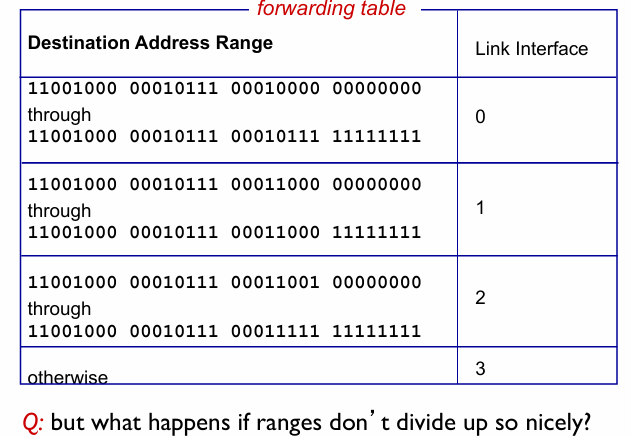
\includegraphics[width=0.6\textwidth]{router_4.1.png}
    \caption{%
        \textbf{Forwarding table con intervalli di indirizzi
       }
        La tabella associa intervalli contigui di indirizzi IP di
        destinazione a interfacce di uscita (0--3). Ogni riga copre
        un blocco di indirizzi scritto in forma binaria esplicita
        con i limiti inferiore e superiore dell'intervallo.
        L'ultima riga \texttt{otherwise} è la \textbf{default route}:
        cattura tutti i datagrammi il cui indirizzo non rientra in
        nessuno degli intervalli precedenti e li invia all'interfaccia~3
        (tipicamente il gateway verso il resto di Internet).
        Le regole vengono usate in ordine (quella più \textbf{in alto} ha precedenza).
        La domanda evidenziata in rosso nella slide -- \textit{``but what
        happens if ranges don't divide up so nicely?''} -- motiva
        direttamente l'introduzione del \textbf{CIDR} e del
        \textbf{Longest Prefix Matching}: gli intervalli reali non sono
        mai perfettamente allineati a potenze di~2, quindi serve una
        notazione a prefisso flessibile invece degli intervalli espliciti.%
    }
    \label{fig:dest_forwarding_table}
\end{figure}
% ============================================================
\subsubsection{Longest Prefix Matching}
% ============================================================

Nel forwarding basato sulla destinazione, la forwarding table associa
\textbf{intervalli di indirizzi IP} a porte di uscita. Poiché gli indirizzi
IPv4 sono a 32~bit, una tabella con un'entry per ogni indirizzo possibile
avrebbe $2^{32} \approx 4.3$ miliardi di righe -- impraticabile. La
soluzione è usare i \textbf{prefissi}.




La forwarding table usa la notazione con asterischi (\texttt{*}) per
indicare i bit \textit{don't care}:

\begin{table}[H] % [h] suggerisce a LaTeX di mettere la tabella "qui" (here)
\centering
\caption{Tabella indirizzi destinazione e corrispettive interfacce link}
\label{tab:indirizzi} % serve per fare \ref{tab:indirizzi} nel testo
\begin{tabular}{clc}
\toprule
\textbf{Entry} & \textbf{Prefisso} & \textbf{Interfaccia} \\
\midrule
0 & \texttt{11001000 00010111 00010{*}{*}{*} {*}{*}{*}{*}{*}{*}{*}{*}{*}} & 0 \\
1 & \texttt{11001000 00010111 00011000 {*}{*}{*}{*}{*}{*}{*}{*}{*}} & 1 \\
2 & \texttt{11001000 00010111 00011{*}{*}{*} {*}{*}{*}{*}{*}{*}{*}{*}{*}} & 2 \\
3 & \texttt{otherwise} & 3 \\
\bottomrule
\end{tabular}
\end{table}

        \textbf{Forwarding table con intervalli di indirizzi.}
        Ogni riga copre un intervallo contiguo di indirizzi di destinazione
        e lo mappa a un'interfaccia di uscita (0--3). L'ultima riga
        ``otherwise'' è la \textit{default route}: se nessuna riga
        corrisponde, il pacchetto viene inoltrato verso l'interfaccia~3
        (gateway di default verso Internet).
        Il problema emerge quando gli intervalli non si dividono in modo
        regolare: il prefisso \hyperref[section:CIDR]{CIDR} risolve questa complessità in modo
        elegante.%


\begin{defbox}{Longest Prefix Matching (LPM)}
Quando si cerca un indirizzo di destinazione nella forwarding table, si
applica la regola del \textbf{prefisso più lungo} (\textit{longest prefix
match}): tra tutte le entry la cui maschera di rete ``copre'' l'indirizzo
cercato, si sceglie quella con il \textbf{maggior numero di bit specificati}
(cioè il prefisso più specifico, con la subnet mask più lunga).

Intuitivamente: è come cercare un indirizzo stradale -- se esiste una regola
specifica per ``Via Roma 5, Bologna'' e una generica per ``Bologna'', si
applica la regola più specifica.
\end{defbox}



\begin{esempiobox}{Longest Prefix Matching -- esempi con wildcard}
NOTA: per gli indirizzi di destinazione vedi tabella 5.6

\textbf{Esempio 1} -- DA =
\texttt{%
    11001000\;00010111\;%
    \colorbox{cyan!30}{00010}110\;10100001%
}

Confronto con le entry:
\begin{itemize}
    \item Entry~0: prefisso \texttt{\colorbox{cyan!30}{00010}***} -- i
          primi 21~bit corrispondono \checkmark
    \item Entry~1: prefisso \texttt{00011000} -- bit 18 differisce
          (\texttt{0} vs \texttt{1}) \texttimes
    \item Entry~2: prefisso \texttt{00011***} -- bit 18 differisce
          (\texttt{0} vs \texttt{1}) \texttimes
\end{itemize}
Un solo match $\Rightarrow$ \textbf{interfaccia~0}.

\vspace{0.4cm}

\textbf{Esempio 2} -- DA =
\texttt{%
    11001000\;00010111\;%
    \colorbox{cyan!30}{00011000}\;10101010%
}

Confronto con le entry:
\begin{itemize}
    \item Entry~0: prefisso \texttt{00010***} -- bit 18 differisce
          (\texttt{1} vs \texttt{0}) \texttimes
    \item Entry~1: prefisso \texttt{\colorbox{cyan!30}{00011000}}***
          -- tutti i 24~bit specificati corrispondono \checkmark
    \item Entry~2: prefisso \texttt{\colorbox{cyan!40}{00011}***}
          -- i 21~bit specificati corrispondono \checkmark
\end{itemize}
Due match: entry~1 (24~bit) ed entry~2 (21~bit).
Si applica il \textbf{longest prefix}: vince entry~1 perché
$24 > 21$ $\Rightarrow$ \textbf{interfaccia~1}.

\vspace{0.3cm}
\begin{center}
\begin{tikzpicture}
    \node[draw=blue!50, fill=cyan!10, rounded corners, inner sep=8pt,
          font=\small, align=center] {
        \textbf{Regola generale}: tra tutte le entry che fanno match,\\
        si sceglie quella con il prefisso \textbf{più lungo} (più specifico).\\
        L'evidenziazione \colorbox{cyan!30}{azzurra} mostra i bit\\
        effettivamente confrontati con la forwarding table.
    };
\end{tikzpicture}
\end{center}

\end{esempiobox}

\begin{notebox}{Implementazione hardware con TCAM}
Il Longest Prefix Matching deve avvenire in \textbf{un solo ciclo di clock}
per rispettare il vincolo line-rate. Questo viene realizzato con memorie
\textbf{TCAM} (\textit{Ternary Content Addressable Memory}):
\begin{itemize}
    \item Nelle RAM normali si fornisce un \textit{indirizzo} e si legge
          il \textit{contenuto}: operazione $O(1)$ ma con un solo accesso
          per volta.
    \item Nelle CAM si fornisce il \textit{contenuto} (o parte di esso) e
          si ottiene l'\textit{indirizzo}: ricerca parallela su tutta la
          memoria in un ciclo.
    \item Le TCAM sono ``ternarie'' perché ogni bit può valere 0, 1 oppure
          \textbf{X} (don't care / wildcard), il che le rende perfette per
          i prefissi di rete.
    \item Un router Cisco Catalyst può contenere circa \textbf{1~milione}
          di entry TCAM, più che sufficiente per la routing table di
          Internet ($\approx 900$K prefissi nel 2024).
\end{itemize}
\end{notebox}


\newpage
% ============================================================
\subsection{Switching Fabric (tipologie)}
% ============================================================

Lo \textbf{switching fabric} è il componente che trasferisce fisicamente i
datagrammi dalle porte di ingresso alle porte di uscita. È il cuore del
router: la sua velocità determina il throughput massimo del dispositivo.

\begin{defbox}{Switching rate}
La velocità dello switching fabric si misura come il numero di datagrammi
(o bit) che può trasferire per unità di tempo. Si esprime spesso come
multiplo della velocità dei singoli link: con $N$ porte a velocità $R$,
la velocità ideale del fabric è $N \times R$ (così ogni porta di ingresso
può trasmettere a piena velocità simultaneamente).
\end{defbox}

Esistono tre tecnologie principali, in ordine crescente di prestazioni:

\begin{figure}[H]
    \centering
    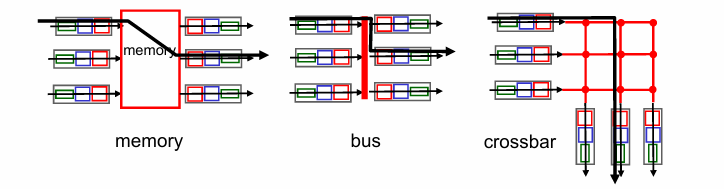
\includegraphics[width=0.88\textwidth]{router_5.png}
    \caption{Le tre tipologie di switching fabric.}
    \label{fig:switching_fabrics}
\end{figure}

Come illustrato nella Figura \ref{fig:switching_fabrics}, le architetture per lo switching fabric si dividono in tre categorie principali:

\begin{itemize}
    \item[\textbf{(a)}] \textbf{Via memoria} (sinistra): le porte di ingresso e di uscita sono collegate a una memoria condivisa. Ogni pacchetto deve compiere due attraversamenti del bus di sistema (dall'ingresso verso la memoria, e successivamente dalla memoria verso l'uscita).
    \item[\textbf{(b)}] \textbf{Via bus} (centro): l'ingresso e l'uscita sono connessi tramite un unico bus condiviso. Questa architettura implica che un solo pacchetto alla volta possa utilizzare il mezzo per il trasferimento.
    \item[\textbf{(c)}] \textbf{Via crossbar / interconnection network} (destra): sfrutta una griglia di $N \times N$ punti di commutazione che consente trasferimenti simultanei di più pacchetti, purché indirizzati su coppie ingresso-uscita differenti. Lo stato (chiusura o apertura) dei punti di incrocio rossi della matrice è programmabile via software.
\end{itemize}















\newpage
% ------- MEMORIA ---------------------------------------------
\subsubsection{a) Switching via memoria}

\begin{figure}[H]
    \centering
    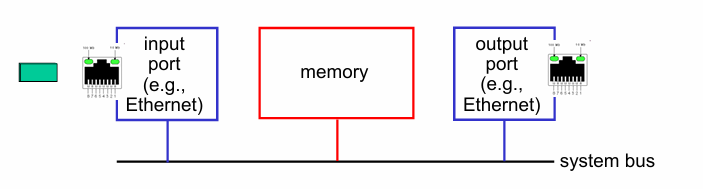
\includegraphics[width=0.72\textwidth]{router_6.png}
    \caption{Switching via memoria in un router di prima generazione.}
    \label{fig:switch_memory}
\end{figure}

Come illustrato nella Figura \ref{fig:switch_memory}, questa architettura (tipica dei router degli anni '80 e '90) delega le operazioni al software, comportandosi essenzialmente come un normale computer dotato di schede di rete. Il suo funzionamento e le sue caratteristiche principali si riassumono in:

\begin{itemize}
    \item \textbf{Percorso del datagramma:} il pacchetto in arrivo sulla porta di ingresso attraversa il bus di sistema per essere copiato nella memoria centrale del router. La CPU (routing processor) ne legge l'header, consulta la forwarding table e lo ricopia dalla memoria alla porta di uscita corretta.
    \item \textbf{Coinvolgimento della CPU:} il processore principale partecipa attivamente all'inoltro di \emph{ogni singolo} pacchetto. Questa dipendenza non permette al sistema di scalare con l'aumento del traffico, limitando le velocità tipiche a pochi Gbps totali.
    \item \textbf{Collo di bottiglia e performance:} il bus di sistema e la banda della memoria rappresentano il limite fisico dell'architettura (\emph{single point of contention}). Ogni pacchetto richiede \textbf{2 attraversamenti del bus} (ingresso $\to$ memoria, memoria $\to$ uscita); di conseguenza, con una capacità del bus pari a $B$~Gbps, la velocità massima effettiva di forwarding sarà dimezzata a $B/2$.
    \item \textbf{Assenza di parallelismo:} l'uso esclusivo di un singolo bus condiviso impedisce i trasferimenti simultanei, anche se rende la progettazione hardware del dispositivo molto semplice da realizzare.
\end{itemize}
% ------- BUS -------------------------------------------------
\newpage
\subsubsection{b) Switching via bus}

\begin{figure}[H]
    \centering
    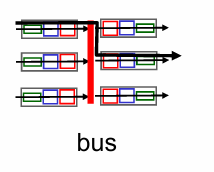
\includegraphics[width=0.5\textwidth]{router_7.png}
    \caption{Architettura di switching tramite bus condiviso.}
    \label{fig:switch_bus}
\end{figure}

Come mostrato nella Figura \ref{fig:switch_bus}, in questa architettura l'inoltro avviene attraverso un bus interno dedicato (rappresentato dalla barra rossa verticale). Il funzionamento e le caratteristiche principali sono i seguenti:

\begin{itemize}
    \item \textbf{Trasferimento diretto e ruolo della CPU:} il datagramma viene trasferito direttamente dalla memoria della porta di ingresso a quella della porta di uscita. La CPU \textbf{non è più coinvolta} nel processo di forwarding, portando un drastico miglioramento delle prestazioni rispetto allo switching via memoria.
    \item \textbf{Meccanismo di inoltro:} la porta di ingresso "prepara" il pacchetto aggiungendo un'etichetta interna che indica la porta di destinazione. Il pacchetto viene poi trasmesso sul bus: tutte le porte di uscita lo ricevono simultaneamente, ma solo quella che corrisponde all'etichetta lo accetta e lo elabora.
    \item \textbf{Bus contention e code:} il problema principale di questa struttura è la contesa del mezzo (\textbf{bus contention}). Essendo il bus condiviso, solo \emph{un} pacchetto alla volta può attraversarlo; eventuali altri datagrammi in arrivo devono aspettare il proprio turno nelle code delle porte di ingresso.
    \item \textbf{Prestazioni e scalabilità:} la velocità massima di switching è strettamente limitata dalla \textbf{banda del bus} (un esempio reale è il router Cisco 5600, dotato di un bus da 32~Gbps). Questa capacità è perfettamente adeguata per router di accesso o per reti aziendali di fascia media, ma non scala a sufficienza per i router di backbone ad altissime prestazioni, dove i colli di bottiglia (\textbf{Bus contetion} )diventerebbero critici all'aumentare delle porte.
\end{itemize}
% ------- CROSSBAR --------------------------------------------
\newpage
\subsubsection{c) Switching via interconnection network (crossbar)}

\begin{figure}[H]
    \centering
    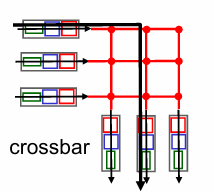
\includegraphics[width=0.4\textwidth]{router_8.png}
    \caption{Architettura di switching via crossbar (rete di interconnessione).}
    \label{fig:switch_crossbar}
\end{figure}

Come illustrato nella Figura \ref{fig:switch_crossbar}, l'architettura via crossbar utilizza una rete di interconnessione per superare i limiti di banda del bus condiviso. Il suo funzionamento e le sue caratteristiche principali si possono riassumere in:

\begin{itemize}
    \item \textbf{Struttura a matrice:} in un crossbar $N \times N$, ogni porta di ingresso è connessa a ogni porta di uscita attraverso uno specifico punto di commutazione (rappresentato dai pallini rossi). Per instradare un datagramma dall'ingresso $i$ all'uscita $j$, il sistema ``chiude'' il punto di incrocio $(i,j)$.
    \item \textbf{Parallelismo dei trasferimenti:} se due o più pacchetti sono diretti verso uscite \emph{diverse}, i rispettivi punti di commutazione si trovano su colonne differenti e possono essere chiusi \textbf{contemporaneamente}. Questo permette trasferimenti totalmente in parallelo. Un conflitto si verifica esclusivamente se due pacchetti tentano di raggiungere la \emph{stessa} porta di uscita nello stesso istante.
    \item \textbf{Elaborazione a celle fisse:} questa è una tecnica avanzata adottata dai router backbone moderni (come ad esempio la serie CISCO 12000). Il datagramma IP a lunghezza variabile viene solitamente frammentato in \textbf{celle di lunghezza fissa} all'ingresso (tecnica ispirata alle celle ATM da 53~byte) per semplificare e velocizzare le operazioni di inoltro, venendo poi riassemblato all'uscita.
    \item \textbf{Scheduling del crossbar:} la decisione su quali connessioni attivare a ogni ciclo, evitando i conflitti tra le porte, costituisce un classico problema di \emph{matching} su grafo bipartito. Viene risolto a livello hardware ricorrendo ad algoritmi di scheduling altamente ottimizzati (come ad esempio l'algoritmo iSLIP).
\end{itemize}
\newpage
\begin{notebox}{Topologie avanzate per switching fabric su silicio}

\begin{figure}[H]
\centering

% ---- (a) ANELLO ----
\begin{subfigure}[t]{0.30\textwidth}
\centering
\begin{tikzpicture}[
    node/.style={circle, draw, fill=unibolight,
                 inner sep=0pt, minimum size=22pt, font=\scriptsize\bfseries},
    scale=1.05
]
\foreach \i in {0,...,7}{
    \node[node] (N\i) at ({90-45*\i}:1.5cm) {\i};
}
\foreach \i in {0,...,7}{
    \pgfmathtruncatemacro{\j}{mod(\i+1,8)}
    \draw[thick, uniboblue] (N\i) -- (N\j);
}
% frecce bidirezionali su un arco per mostrare le due strade
\draw[->, thick, red!70, bend left=20]  (N0) to (N4);
\draw[->, thick, red!70, bend right=20] (N0) to (N4);
\node[font=\tiny, text=red!70] at (0,-0.05) {\textit{2 paths}};
\end{tikzpicture}
\caption*{\textbf{(a) Anello (ring)}}
\end{subfigure}
\hfill
% ---- (b) SPIDERGON ----
\begin{subfigure}[t]{0.34\textwidth}
\centering
\begin{tikzpicture}[
    node/.style={circle, draw, fill=unibolight,
                 inner sep=0pt, minimum size=22pt, font=\scriptsize\bfseries},
    scale=1.05
]
\foreach \i in {0,...,7}{
    \node[node] (N\i) at ({90-45*\i}:1.5cm) {\i};
}
% link ad anello
\foreach \i in {0,...,7}{
    \pgfmathtruncatemacro{\j}{mod(\i+1,8)}
    \draw[thick, uniboblue] (N\i) -- (N\j);
}
% link diametrali (ogni nodo i -- nodo i+4)
\foreach \i in {0,...,3}{
    \pgfmathtruncatemacro{\j}{\i+4}
    \draw[thick, okgreen, dashed] (N\i) -- (N\j);
}
% legenda
\node[font=\tiny, text=okgreen] at (0,-2.1)
    {--- link diametrale ($i \leftrightarrow i{+}N/2$)};
\end{tikzpicture}
\caption*{\textbf{(b) Spidergon}}
\end{subfigure}
\hfill
% ---- (c) MESH TOROIDALE ----
\begin{subfigure}[t]{0.30\textwidth}
\centering
\begin{tikzpicture}[
    node/.style={circle, draw, fill=unibolight,
                 inner sep=0pt, minimum size=18pt, font=\tiny\bfseries},
    scale=0.78
]
% 4x4 grid
\foreach \r in {0,...,3}{
    \foreach \c in {0,...,3}{
        \pgfmathtruncatemacro{\idx}{4*\r+\c}
        \node[node] (N\r\c) at ({\c*1.4},{-\r*1.4}) {\idx};
    }
}
% link orizzontali interni
\foreach \r in {0,...,3}{
    \foreach \c in {0,...,2}{
        \pgfmathtruncatemacro{\cn}{\c+1}
        \draw[thick, uniboblue] (N\r\c) -- (N\r\cn);
    }
}
% link verticali interni
\foreach \c in {0,...,3}{
    \foreach \r in {0,...,2}{
        \pgfmathtruncatemacro{\rn}{\r+1}
        \draw[thick, uniboblue] (N\r\c) -- (N\rn\c);
    }
}
% wrap-around orizzontali (rosso tratteggiato = difficile su silicio)
\foreach \r in {0,...,3}{
    \draw[thick, alertred, dashed, bend left=45] (N\r 3) to (N\r 0);
}
% wrap-around verticali
\foreach \c in {0,...,3}{
    \draw[thick, alertred, dashed, bend right=45] (N3\c) to (N0\c);
}
\node[font=\tiny, text=alertred] at (2.1,-4.8)
    {--- wrap-around (difficile su chip)};
\end{tikzpicture}
\caption*{\textbf{(c) Mesh toroidale $4{\times}4$}}
\end{subfigure}

\caption{%
    \textbf{Topologie di switching fabric su silicio (Network-on-Chip):   }
    \textbf{(a) Anello}: 8 nodi in cerchio, grado~2. Ogni coppia ha
    esattamente due percorsi alternativi (orario e antiorario, frecce
    rosse). Semplicissimo da realizzare su chip. Costo medio $N/4$ hop.
    \textbf{(b) Spidergon}: estende l'anello con un collegamento
    diametrale (linea verde tratteggiata) tra ogni nodo $i$ e il nodo
    $i + N/2$ opposto. Il diametro si dimezza rispetto all'anello puro
    ($N/8$ invece di $N/4$), mantenendo il grado~3 e la semplicità di
    layout.
    \textbf{(c) Mesh toroidale $4\times4$}: griglia con wrap-around --
    i nodi al bordo sono connessi ai nodi sul bordo opposto (linee rosse
    tratteggiate). Diametro $\sqrt{N}$, grado~4. Il wrap-around rende il
    layout fisico del chip molto più complesso: i collegamenti che
    ``scavalcano'' il chip hanno lunghezze di filo eterogenee, causando
    problemi di timing e consumo energetico.%
}
\label{fig:noc_topologies}
\end{figure}
Le tre architetture classiche non esauriscono il panorama delle soluzioni
reali. Nei sistemi \textbf{Network-on-Chip} (NoC) -- dove il fabric è
integrato direttamente su un singolo chip -- emergono ulteriori topologie,
ognuna con un diverso trade-off tra costo di realizzazione, latenza e
tolleranza ai guasti.


\vspace{0.5cm}
\textbf{Topologia ad anello (\textit{ring})}

I nodi sono disposti in cerchio; ogni nodo è connesso solo ai due vicini
immediati (sinistro e destro).
\begin{itemize}
    \item \textbf{Vantaggio}: molto più semplice da realizzare su silicio
          rispetto alla mesh toroidale -- tutti i collegamenti hanno
          lunghezza simile e il layout è regolare. Offre
          \textbf{due percorsi alternativi} tra qualsiasi coppia di nodi
          (senso orario e antiorario), il che fornisce una forma di
          tolleranza ai guasti.
    \item \textbf{Svantaggio}: il costo medio di un trasferimento cresce
          linearmente con il numero di nodi. Con $N$ nodi, il numero
          medio di hop è $N/4$ (percorso ottimo su anello), che per $N$
          grande diventa proibitivo. Esempio: con 64 nodi, un pacchetto
          attraversa in media 16 nodi prima di arrivare a destinazione.
\end{itemize}

\vspace{0.3cm}
\textbf{Topologia Spidergon}

La Spidergon è una topologia ibrida che estende l'anello aggiungendo
collegamenti diametrali: ogni nodo $i$ è connesso, oltre ai vicini
adiacenti sull'anello, anche al nodo ``opposto'' $i + N/2$.
\begin{itemize}
    \item \textbf{Vantaggio}: il collegamento diametrale dimezza
          il diametro della rete rispetto all'anello puro, abbattendo
          il costo medio da $N/4$ a $N/8$ hop. Mantiene la semplicità
          di layout dell'anello (tutti i nodi hanno lo stesso grado~3)
          ed è facilmente scalabile.
    \item \textbf{Svantaggio}: il collegamento diametrale, pur più
          corto di quello toroidale, introduce comunque una variazione
          di lunghezza rispetto ai link adiacenti; per $N$ molto grandi
          rimane comunque un costo $O(N)$.
\end{itemize}


\vspace{0.cm}
\textbf{Topologia toroidale (mesh toroidale)}

Una griglia $N \times N$ in cui i nodi al bordo sono collegati ai nodi
sul bordo opposto, eliminando i ``bordi aperti'' della mesh piatta(detta anche griglia piatta).
\begin{itemize}
    \item \textbf{Vantaggio}: percorsi più corti e bilanciati rispetto
          alla mesh piatta; diameter ridotto.
    \item \textbf{Svantaggio}: difficile da realizzare su silicio --
          i collegamenti che ``scavalcano'' il chip (wrap-around) hanno
          lunghezze di filo molto diverse, causando problemi di timing
          e consumo energetico. Rende il layout fisico del chip
          notevolmente più complesso.
\end{itemize}

\vspace{0.3cm}

\begin{center}
\begin{tabular}{lccc}
\toprule
\textbf{Topologia} & \textbf{Grado nodo} & \textbf{Diametro}
    & \textbf{Complessità layout} \\
\midrule
Anello        & 2 & $N/2$   & Bassa \\
Spidergon     & 3 & $N/4$   & Medio-bassa \\
Mesh toroidale & 4 & $\sqrt{N}$ & Alta \\
Crossbar      & $N$ & 1      & Molto alta ($O(N^2)$ link) \\
\bottomrule
\end{tabular}
\end{center}

\subsection*{Definizione dei parametri topologici}

Nel contesto delle reti e dei Network-on-Chip (NoC), i termini \emph{grado} e \emph{diametro} derivano dalla teoria dei grafi, ma assumono un'importanza pratica fondamentale per la progettazione hardware e le prestazioni del sistema.

\subsubsection*{1. Grado del nodo (Node Degree)}
\begin{itemize}
    \item \textbf{Significato teorico:} indica il numero di collegamenti diretti (archi) che entrano o escono da un singolo nodo.
    \item \textbf{Significato nel mondo reale:} corrisponde al \textbf{numero di porte fisiche} di input e output che il singolo router o elemento di switching deve possedere.
    \item \textbf{Impatto architetturale:} un grado più elevato richiede un hardware più complesso, una maggiore occupazione di area sul chip di silicio e un consumo energetico superiore. Per questo motivo, nella progettazione si cerca spesso un compromesso per minimizzarlo.
\end{itemize}

\subsubsection*{2. Diametro della rete (Network Diameter)}
\begin{itemize}
    \item \textbf{Significato teorico:} rappresenta il percorso minimo più lungo tra tutte le possibili coppie di nodi nella rete (ovvero, il massimo numero di "salti" o \emph{hop} necessari nel caso peggiore).
    \item \textbf{Significato nel mondo reale:} corrisponde alla \textbf{latenza massima garantita (worst-case latency)}.
    \item \textbf{Impatto architetturale:} un diametro basso è cruciale per le prestazioni, poiché assicura che anche i nodi fisicamente o logicamente più lontani possano comunicare velocemente con un numero limitato di attraversamenti.
\end{itemize}


\end{notebox}


\newpage

\subsection{Riepilogo comparativo delle tre architetture
    di switching fabric}
\begin{tcolorbox}[colback=unibolight, colframe=uniboblue,
    title=\bfseries Riepilogo comparativo delle tre architetture
    di switching fabric, breakable]
\small
\renewcommand{\arraystretch}{1.6}
\begin{tabularx}{\textwidth}{p{2.0cm} X X}
\toprule
\textbf{Tipo}
    & \textbf{Vantaggi}
    & \textbf{Svantaggi e bottleneck} \\
\midrule

\textbf{Memoria}
\newline
{\footnotesize\textit{1 pkt/volta}}
    &
    Semplicissimo: nessun hardware dedicato,
    architettura identica a un comune PC con
    schede di rete.
    Adatto a router di prima generazione.
    &
    \textbf{Bottleneck}:
    - banda del bus di sistema.
    Ogni pacchetto richiede \textbf{2 bus crossing}
    obbligatori (ingresso $\to$ memoria, memoria
    $\to$ uscita), quindi il throughput massimo
    è $B_{\text{bus}}/2$.
    
    - CPU coinvolta per ogni singolo pacchetto:
    non scala con il traffico.
    Velocità tipica: pochi Gbps totali.
    \\

\textbf{Bus}
\newline
{\footnotesize\textit{1 pkt/volta}}
    &
    CPU \emph{non} coinvolta nel forwarding:
    un solo bus crossing per datagramma.
    Costo contenuto, sufficiente per reti
    di accesso e aziendali.
    Esempio reale: Cisco~5600, bus~32~Gbps.
    &
    \textbf{Bottleneck}: \textit{bus contention}.
    Il bus è condiviso tra tutte le porte:
    un solo pacchetto per volta può
    attraversarlo. Tutti gli altri attendono
    in coda all'ingresso.
    Non scala oltre $\sim$100~Gbps:
    aumentare il numero di porte non
    aumenta il throughput.
    \\

\textbf{Crossbar}
\newline
{\footnotesize\textit{fino a $N$ pkt/volta}}
    &
    Trasferimenti \textbf{paralleli}: più
    coppie ingresso-uscita \emph{distinte}
    comunicano simultaneamente.
    I datagrammi vengono frammentati in
    celle a lunghezza fissa per semplificare
    l'arbitraggio.
    Scala fino a Tbps.
    Esempio reale: Cisco~12000, 60~Gbps.
    &
    \textbf{Bottleneck}: \textit{output port contention}.
    Se due o più pacchetti puntano alla
    \emph{stessa} porta di uscita nello
    stesso ciclo, uno solo passa e gli altri
    aspettano -- da qui l'HOL blocking
    alle porte di ingresso.
    Complessità hardware $O(N^2)$;
    scheduling complesso (matching su grafo
    bipartito, es.\ algoritmo~iSLIP);
    costo elevato.
    \\

\bottomrule
\end{tabularx}

\end{tcolorbox}

\newpage
% ============================================================
\subsection{Accodamento all'ingresso e HOL Blocking}
% ============================================================

Anche con uno switching fabric veloce, possono formarsi code alle porte di
ingresso. Il caso critico è quando il fabric è \textbf{più lento della somma
delle velocità di tutti i link di ingresso}: i datagrammi si accumulano in
attesa di essere commutati.

\begin{figure}[H]
    \centering
    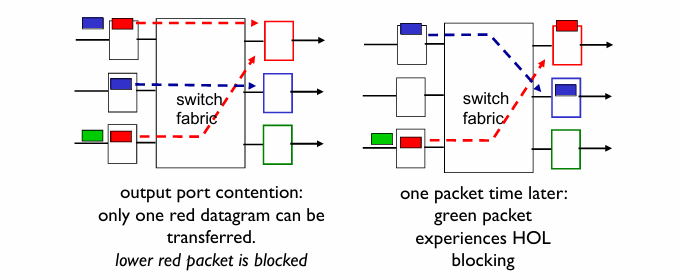
\includegraphics[width=0.88\textwidth]{router_9.png}
    \caption{Accodamento alle porte di ingresso e fenomeno dell'Head-of-Line (HOL) blocking.}
    \label{fig:hol_blocking}
\end{figure}

Come illustrato nella Figura \ref{fig:hol_blocking}, l'accodamento dei pacchetti sulle porte di ingresso può portare a inefficienze di rete, descritte attraverso la seguente sequenza:

\begin{itemize}
    \item \textbf{Situazione iniziale (sinistra):} tre porte di ingresso presentano dei pacchetti in coda. I due pacchetti rossi (situati in testa alla prima e alla terza coda) devono essere instradati verso la stessa porta di uscita. Poiché lo switching fabric può servire \emph{un solo} pacchetto alla volta verso una specifica destinazione, il secondo pacchetto rosso viene bloccato e trattenuto.
    \item \textbf{Conseguenza (destra):} un istante temporale dopo, il pacchetto verde -- che si trova fisicamente accodato \emph{dietro} al secondo pacchetto rosso nella terza coda -- vorrebbe procedere verso la propria porta di uscita (che risulta attualmente libera). Tuttavia, \textbf{non può avanzare} perché il pacchetto rosso in testa alla sua coda non è ancora stato servito.
    \item \textbf{Definizione di HOL blocking:} questa specifica dinamica prende il nome di \textbf{Head-of-Line blocking}. Si verifica ogniqualvolta il pacchetto in \emph{testa} a una coda blocca l'elaborazione dei pacchetti posizionati dietro di lui, impedendone l'inoltro anche se le loro rispettive porte di destinazione sarebbero libere e disponibili.
\end{itemize}

\begin{urgentbox}{HOL Blocking -- impatto sulle prestazioni}
Il Head-of-Line Blocking non è solo un inconveniente teorico: analisi
formali dimostrano che con traffico casuale uniforme e un crossbar ideale,
l'HOL blocking da solo limita il throughput massimo del fabric a circa il
\textbf{58.6\%} della capacità nominale. Soluzioni pratiche includono:
\begin{itemize}
    \item \textbf{Virtual Output Queuing (VOQ)}: invece di una sola coda
          per porta di ingresso, si mantengono $N$ code virtuali separate
          (una per ciascuna porta di uscita). Un pacchetto non blocca mai
          pacchetti destinati ad uscite diverse.
    
\end{itemize}
\end{urgentbox}

\newpage
% ============================================================
\subsection{ Accodamento Porte di uscita (\textit{Output Ports})}
% ============================================================

Le porte di uscita ricevono i datagrammi dallo switching fabric, li accodano
e li trasmettono sul link fisico. Anche qui possono formarsi code, stavolta
per ragioni diverse.

\begin{figure}[H]
    \centering
    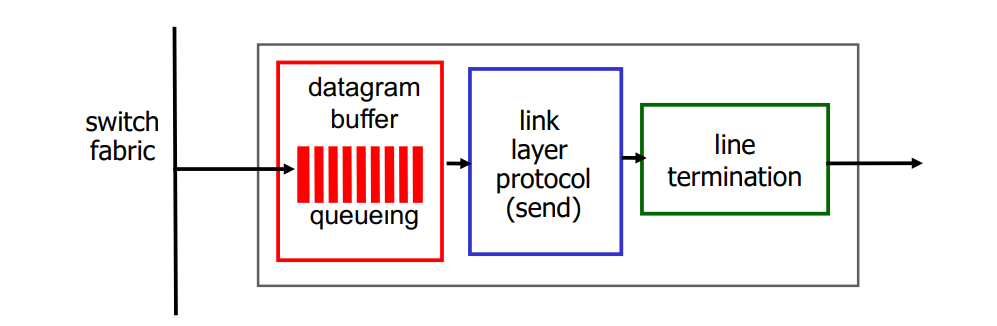
\includegraphics[width=0.82\textwidth]{router_10.png}
    \caption{Struttura interna di una porta di uscita.}
    \label{fig:output_port}
\end{figure}

Come illustrato nella Figura \ref{fig:output_port}, l'elaborazione dei pacchetti in uscita attraversa tre stadi principali, affiancati da un meccanismo di controllo:

\begin{enumerate}
    \item \textbf{Datagram buffer} (riquadro rosso con barre verticali): i datagrammi in arrivo dallo switching fabric (da sinistra) vengono ricevuti e temporaneamente accodati in questo buffer di attesa.
    \item \textbf{Scheduling\footnote{Vedremo nella sezione \ref{scheduling}}}: un meccanismo dedicato (indicato dalla freccia che va dalla coda al blocco link) interviene per decidere l'ordine di inoltro, stabilendo quale datagramma trasmettere per primo quando vi sono più pacchetti in attesa nel buffer.
    \item \textbf{Link layer protocol} (riquadro blu): si occupa della preparazione logica per l'invio sul mezzo condiviso. In questa fase viene aggiunto l'header del frame data-link e vengono applicate le regole del protocollo MAC (ad esempio, l'incapsulamento Ethernet).
    \item \textbf{Line termination} (riquadro verde): costituisce l'ultimo stadio e opera a livello fisico, convertendo la sequenza di bit appena creata nei segnali fisici veri e propri destinati a viaggiare sul link uscente.
\end{enumerate}

\newpage
\begin{notebox}{Code e perdita di pacchetti: Input vs. Output}
Una domanda frequente è: i pacchetti si perdono alle porte di \emph{ingresso} o di \emph{uscita}? Per rispondere correttamente, occorre separare le cause strutturali che generano congestione nei due diversi punti del router.

\vspace{0.2cm}
\textbf{1. Congestione alle porte di USCITA (Lo scenario dominante)}
La perdita di pacchetti in Internet si manifesta quasi esclusivamente qui. Si verifica quando la \textbf{velocità di arrivo dei datagrammi dal fabric supera la velocità di trasmissione del link}.
\begin{itemize}
    \item \textbf{Causa (Asimmetria del traffico):} se $N$ porte di ingresso inviano simultaneamente traffico verso la \emph{stessa} porta di destinazione, un fabric moderno ed efficiente (es.\ crossbar) recapiterà all'uscita $N$ pacchetti per ciclo. Tuttavia, il link fisico in uscita può trasmetterne solo 1 per volta alla sua velocità fissa $R$. Il buffer, di conseguenza, inizia a riempirsi.
    \item \textbf{Effetto a cascata sul TCP:} l'accumulo di pacchetti fa crescere a dismisura il ritardo di coda. Questo può far scadere prematuramente il \textbf{timer di ritrasmissione} del protocollo TCP: il mittente inietta \textbf{duplicati in rete}, aggravando la congestione. Quando il buffer si satura definitivamente, i pacchetti in eccesso vengono scartati (\emph{packet drop}). Questa perdita è proprio il segnale che il TCP utilizza per rilevare la congestione e dimezzare la propria finestra di trasmissione\footnote{Come visto nel CAP 3 sezione 3.4.7 (Sliding Window)}.
\end{itemize}

\vspace{0.2cm}
\textbf{2. Congestione alle porte di INGRESSO (Scenari minoritari)}
L'accodamento in ingresso è raro nei router moderni di fascia alta e dipende da limiti intrinseci dell'hardware del dispositivo, non dalle dinamiche del traffico globale.
\begin{itemize}
    \item \textbf{Causa hardware (Fabric sottodimensionato):} si forma una coda in ingresso se l'architettura interna dello switch è troppo lenta (capacità inferiore alla somma delle velocità dei link in entrata) e non riesce a smaltire i pacchetti in tempo reale.
    \item \textbf{Causa logica (HOL Blocking):} il pacchetto in \emph{testa} a una coda, in attesa che la propria uscita si liberi, blocca fisicamente l'elaborazione dei pacchetti dietro di lui, anche qualora le loro porte di destinazione fossero libere. È un problema logico noto come \textbf{Head-of-Line blocking}, oggi ampiamente risolto tramite l'implementazione di code virtuali (VOQ, \textit{Virtual Output Queuing}).
\end{itemize}

\vspace{0.1cm}
In sintesi: le code in \textbf{ingresso} indicano che il router sta faticando internamente, mentre le code in \textbf{uscita} (quelle che portano alla perdita reale di dati) indicano che la rete stessa è congestionata.
\end{notebox}

\begin{collegamentobox}
\textbf{Congestione nei buffer di uscita e risposta di TCP
-- collegamento con il Capitolo~3}
\vspace{1cm}

Come discusso in dettaglio nella
\textbf{Sezione~3.4.5} (Controllo della congestione) e nella
\textbf{Sezione~3.4.7} (Sliding Window), TCP reagisce alla perdita di
pacchetti modificando dinamicamente la propria \textbf{finestra
scorrevole SW}:

\begin{itemize}
    \item \textbf{Causa scatenante}: il buffer di uscita di un router
          congestionato si riempie e scarta datagrammi. Il mittente TCP
          non riceve l'ACK corrispondente entro il timeout.

    \item \textbf{Risposta di TCP -- Timeout}:
          $\text{SW} \leftarrow 1$ (\textit{Slow Start}).
          La finestra viene azzerata a 1 pacchetto sonda e ricresce
          esponenzialmente ($\text{SW} \leftarrow 2\,\text{SW}$) fino
          a metà della soglia critica precedente, dopodiché la crescita
          diventa lineare (\textit{Congestion Avoidance},
          $\text{SW} \leftarrow \text{SW} + 1$).

    \item \textbf{Vincolo combinato}: in ogni istante il numero di
          segmenti ``in volo'' è limitato da entrambi i controlli
          \[
              \text{SW} \;\leq\; \text{RB}
          \]
          dove \textbf{RB} (Receive Buffer, dichiarato dal ricevitore
          in ogni segmento TCP) governa il \textit{controllo di flusso}
          verso il destinatario finale (Sezione~3.4.6), mentre
          \textbf{SW} governa il \textit{controllo della congestione}
          verso la rete. I due meccanismi operano in parallelo e in
          modo indipendente.

    \item \textbf{Indipendenza delle sorgenti}: come evidenziato nella
          Sezione~3.4.7, le varie connessioni TCP che attraversano lo
          stesso router congestionato sono completamente non coordinate.
          Mentre una sorgente rileva la perdita e azzera SW, altre
          potrebbero simultaneamente trovarsi in fase di crescita
          esponenziale -- questo spiega perché la congestione tende a
          ripresentarsi ciclicamente anche dopo che una sorgente ha
          rallentato.
\end{itemize}

\end{collegamentobox}

\newpage
\begin{figure}[H]
    \centering
    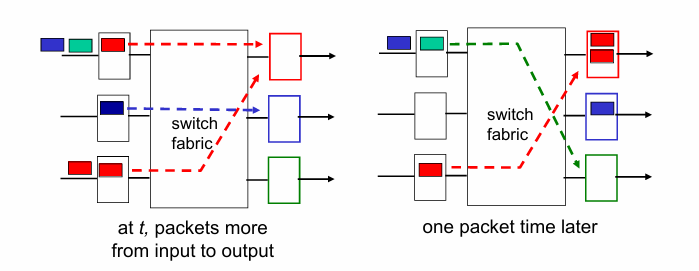
\includegraphics[width=0.88\textwidth]{router_11.png}
    \caption{Accodamento alle porte di uscita (Output port queueing) ed evoluzione temporale.}
    \label{fig:output_queueing_time}
\end{figure}

Come illustrato nella Figura \ref{fig:output_queueing_time}, l'accodamento sulle porte di uscita si verifica quando lo \textit{switching fabric} è sufficientemente performante da trasferire più pacchetti verso la medesima destinazione nello stesso slot temporale. La dinamica si sviluppa in due fasi:

\begin{itemize}
    \item \textbf{All'istante $t$ (sinistra):} due pacchetti rossi, posizionati in testa alla prima e alla terza coda di ingresso, sono entrambi destinati alla stessa porta di uscita (quella in alto). A differenza di quanto accade con l'HOL blocking, il fabric è in grado di processare e trasferire \emph{entrambi} i pacchetti simultaneamente senza creare colli di bottiglia all'ingresso.
    \item \textbf{Un istante temporale successivo (destra):} i due pacchetti rossi sono stati trasferiti con successo e si trovano ora \textbf{accodati nel buffer della porta di uscita}, in attesa di essere trasmessi in modo seriale sul link fisico (che può inviare un solo pacchetto alla volta). Nel frattempo, il fabric processa immediatamente i pacchetti che erano in attesa nelle code di ingresso (il pacchetto verde viene instradato verso l'uscita in basso, mentre un nuovo pacchetto rosso va verso l'uscita in alto).
\end{itemize}

Questa architettura elimina il problema dell'Head-of-Line blocking, ma sposta fisiologicamente la congestione sulle porte di uscita. Rende perciò necessari:
 \begin{itemize}
     \item buffer molto capienti in uscita per assorbire i picchi di traffico 

      \item 
algoritmi di \textit{scheduling} per gestire l'ordine effettivo di trasmissione.

 \end{itemize}

\newpage

\subsection{Quanta memoria di buffer serve nelle porte di output?}

La dimensione del buffer di uscita è un parametro critico di progetto.

Buffer troppo piccoli causano perdita di pacchetti;

buffer troppo grandi
aumentano il ritardo (\textit{bufferbloat}).

\begin{defbox}{Dimensionamento dei Buffer: Regola Classica vs. Moderna}
Il calcolo della dimensione ottimale del buffer in uscita ($B$) è un fattore critico per le prestazioni della rete. Nel tempo, le linee guida si sono evolute per riflettere il comportamento aggregato del traffico TCP.

\textbf{1. Regola classica (RFC 3439)}
Progettata originariamente per garantire che il link rimanga pienamente utilizzato anche in attesa degli ACK, evitando che il buffer si svuoti durante un intero Round-Trip Time.
\[
    B = \text{RTT} \times C
\]
\begin{itemize}
    \item \textbf{Parametri:} $\text{RTT}$ è il tempo di andata e ritorno tipico (es.\ circa 250~ms per tratte intercontinentali), $C$ è la capacità del link.
    \item \textbf{Esempio:} Per un link da 10~Gbps, il buffer richiesto è enorme: $B = 0.250 \times 10 \times 10^9 = 2.5$~Gbit.
\end{itemize}

\vspace{0.1cm}
\textbf{2. Raccomandazione moderna (Multiplexing Statistico)}
Sui router moderni transitano migliaia di flussi TCP contemporaneamente. Poiché le loro fasi di congestione sono indipendenti e si distribuiscono nel tempo (\textit{statistical multiplexing}), i picchi si compensano a vicenda, richiedendo buffer drasticamente più piccoli.
\[
    B = \frac{\text{RTT} \times C}{\sqrt{N}}
\]
\begin{itemize}
    \item \textbf{Parametri:} $N$ rappresenta il numero di flussi TCP attivi indipendenti.
    \item \textbf{Esempio:} Mantenendo il link a 10~Gbps e l'RTT a 250~ms, ma con $N = 10.000$ flussi attivi, la necessità crolla a $B \approx 25$~Mbit (ben 100 volte in meno rispetto alla regola classica).
\end{itemize}
\end{defbox}

\begin{notebox}{Il paradosso del Bufferbloat}
Dotare i router di memorie eccessivamente grandi genera un grave problema prestazionale noto come \textbf{bufferbloat} (gonfiore del buffer).

Questo fenomeno si basa su due dinamiche:
\begin{itemize}
    \item \textbf{L'inganno al protocollo TCP:} il TCP rileva la congestione (e rallenta la trasmissione) solo quando un pacchetto viene scartato (\emph{packet drop}). Se il buffer è gigantesco, il router non scarta nulla ma accoda tutto. Il TCP, credendo che la rete sia libera, continua a trasmettere a piena velocità.
    \item \textbf{Il crollo della reattività:} i pacchetti non si perdono, ma rimangono intrappolati in coda per decine o centinaia di millisecondi. Questo "ingorgo" genera ritardi enormi (\emph{lag}), distruggendo le prestazioni di tutte le applicazioni interattive o in tempo reale (gaming, videochiamate, VoIP).
\end{itemize}

In sintesi, un buffer troppo grande privilegia il salvataggio del pacchetto a discapito della latenza. Per questo motivo i router moderni (tramite algoritmi come \textbf{CoDel}) preferiscono scartare intenzionalmente i pacchetti se il tempo di attesa in coda supera una soglia limite, forzando così il TCP a rallentare.
\end{notebox}

\newpage

\subsection{Politiche di cestinamento pacchetti (discard)}
Quando il buffer di uscita è pieno e arriva un nuovo pacchetto, si deve
decidere quale pacchetto scartare. La \textbf{politica di discard (esempi reali)}
determina questa scelta:

\begin{itemize}
    \item \textbf{Tail drop}: si scarta il pacchetto \emph{appena
          arrivato}, senza toccare quelli già in coda. È la politica
          più semplice e la più diffusa. Ha però un difetto noto:
          quando il buffer è costantemente pieno, tutte le connessioni
          TCP che lo attraversano ricevono il segnale di congestione
          (timeout) \emph{simultaneamente} e azzerano tutte insieme
          la propria SW -- il traffico crolla, il buffer si svuota,
          poi tutte ricrescono insieme e lo risaturano. Questo
          fenomeno si chiama \textbf{sincronizzazione globale TCP}
          (\textit{TCP global synchronization}) e causa oscillazioni
          periodiche del throughput.

    \item \textbf{Priority drop}: si scarta il pacchetto con la
          \textbf{priorità più bassa} tra quelli già presenti in coda,
          anche se è arrivato prima di altri. Richiede che i pacchetti
          siano classificati (es.\ tramite il campo DSCP dell'header
          IP). Protegge il traffico a alta priorità (VoIP, video) a
          scapito di quello bulk (download, backup).

    \item \textbf{Random Early Detection (RED)}:  Il pacchetto da scartare
          viene scelto \emph{casualmente} tra quelli in coda.

          RED risolve due problemi distinti rispetto al tail drop:
          \begin{itemize}
              \item \textbf{Evita la sincronizzazione TCP}: poiché i
                    pacchetti vengono scartati casualmente tra
                    connessioni diverse, i segnali di congestione
                    vengono distribuiti nel tempo su sorgenti diverse
                    -- non tutte le connessioni reagiscono insieme.
              \item \textbf{Fairness}: la selezione casuale fa sì che
                    connessioni che inviano più traffico (e quindi
                    hanno più pacchetti in coda) abbiano
                    \emph{proporzionalmente} più probabilità di essere
                    colpite dallo scarto -- chi occupa più risorse
                    viene penalizzato di più, in modo automatico e
                    senza classificazione esplicita.
          \end{itemize}
\end{itemize}
\newpage
% ============================================================
\subsection{Meccanismi di scheduling dell'uscita}
% ============================================================
\label{scheduling}
Lo \textbf{scheduling} è la politica con cui la porta di uscita sceglie
quale datagramma trasmettere per primo quando il buffer contiene più
pacchetti in attesa. È una componente critica per la \textbf{Quality of
Service (QoS)}. 

Mentre le politiche di \emph{discard} si occupano di scegliere quali pacchetti sacrificare per fare spazio quando la coda è satura, lo scheduling determina esclusivamente l'ordine di invio. Le quattro tipologie principali di scheduling sono:

\begin{enumerate}
    \item \textbf{FIFO (First In, First Out):} è l'approccio più semplice e basilare. I pacchetti vengono accodati e trasmessi nell'esatto ordine cronologico in cui sono arrivati al buffer. Non offre alcuna differenziazione per tipo di traffico o priorità.
    
    \item \textbf{Priority Scheduling:} il traffico in arrivo viene classificato e smistato in code distinte per livello di importanza (es.\ alta, media, bassa). Il router serve \emph{sempre} prima la coda a priorità più alta, passando alle successive solo quando questa è completamente vuota. Espone il traffico a bassa priorità al rischio di \textit{starvation} (blocco indefinito).
    
    \item \textbf{Round Robin (RR):} i pacchetti vengono divisi in classi, ma il router le scansiona ciclicamente in modo paritario. Trasmette un pacchetto dalla classe 1, poi uno dalla classe 2, e così via. Garantisce un'equità di base (nessuna classe va in \textit{starvation}), ma non tiene conto della diversa importanza o dimensione dei pacchetti.
    
    \item \textbf{Weighted Fair Queuing (WFQ):} è un'evoluzione del Round Robin. I pacchetti vengono divisi in code a cui è assegnato un \emph{peso} specifico. Il router serve le code in modo ciclico ma \textbf{proporzionale ai pesi} assegnati, garantendo a ogni tipo di traffico una frazione minima di banda senza mai bloccare del tutto nessuna classe.

\end{enumerate}
% ------- FIFO -----------------------------------------------
\subsubsection{1) FIFO (First In, First Out)}

\begin{figure}[H]
    \centering
    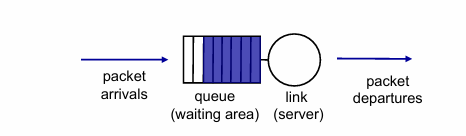
\includegraphics[width=0.76\textwidth]{router_12.png}
    \caption{%
        \textbf{Scheduling FIFO.}
        I pacchetti vengono trasmessi nell'esatto ordine di arrivo in coda.
        Il diagramma mostra l'area di attesa (buffer) e il ``server''
        (link di uscita): i pacchetti passano da sinistra a destra in
        ordine numerico (1, 2, 3, 4, 5). Non c'è differenziazione: tutti
        i pacchetti, indipendentemente da priorità o tipo di traffico,
        vengono trattati allo stesso modo. È il meccanismo più semplice
        e ancora il più diffuso nelle reti domestiche e di accesso.%
    }
    \label{fig:fifo_scheduling}
\end{figure}



% ------- PRIORITY -------------------------------------------
\subsubsection{2) Priority Scheduling}

\begin{figure}[H]
    \centering
    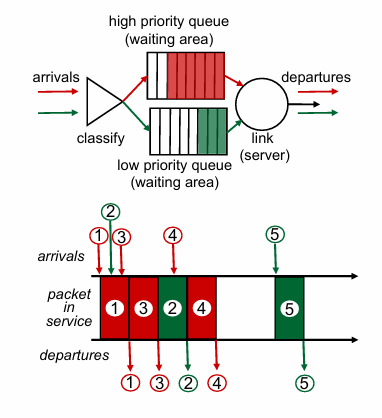
\includegraphics[width=0.5\textwidth]{router_13.png}
    \caption{%
        \textbf{Priority Scheduling con due classi.}
        I pacchetti in arrivo vengono \textbf{classificati} (blocco
        triangolare) e smistati in due code separate: alta priorità
        (coda rossa, in alto) e bassa priorità (coda verde, in basso).
        Il link serve \emph{sempre} la coda ad alta priorità finché non è
        vuota; solo allora passa alla coda bassa.

        
    }
    \label{fig:priority_scheduling}
\end{figure}

        Il diagramma temporale in basso mostra l'ordine di trasmissione:
        i pacchetti 1 e 3 (rossi, alta priorità) vengono trasmessi
        immediatamente; il pacchetto~2 (verde) viene servito dopo il
        pacchetto~3 (rosso, alta priorità) nonostante sia arrivato prima,
        semplicemente perché ha classe superiore.%
        
\vspace{1cm}
La classificazione può basarsi su qualsiasi campo dell'header IP (o TCP/UDP):
indirizzo sorgente/destinazione, valore del campo DSCP (\textit{Differentiated
Services Code Point}), numero di porta. In ambito aziendale è comune dare
alta priorità al traffico VoIP o video-conferenza rispetto al traffico
dati bulk (download, backup).

\begin{urgentbox}{Starvation nel priority scheduling}
Il priority scheduling puro ha un difetto grave: se la coda ad alta
priorità non si svuota mai (perché il traffico ad alta priorità arriva
continuamente), i pacchetti a bassa priorità \textbf{non vengono mai
serviti} (\textit{starvation}). 

Soluzioni: \textit{aging} (aumentare
gradualmente la priorità dei pacchetti che aspettano troppo a lungo) oppure
usare WFQ con pesi molto diversi invece del priority puro.
\end{urgentbox}

% ------- ROUND ROBIN ----------------------------------------
\subsubsection{Round Robin (RR)}

\begin{figure}[H]
    \centering
    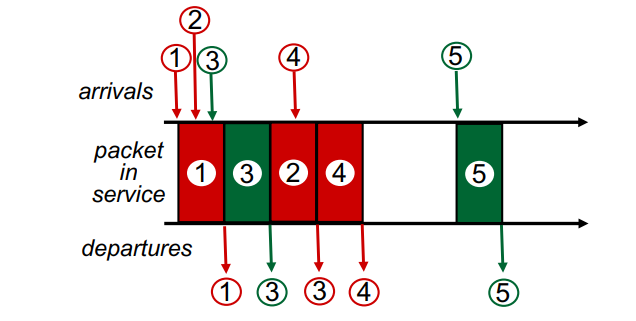
\includegraphics[width=0.82\textwidth]{router_14.png}
    \caption{%
        \textbf{Round Robin Scheduling.}
        Il server scansiona ciclicamente le classi: invia un pacchetto
        completo dalla classe~1, poi uno dalla classe~2, poi uno dalla
        classe~3, poi ritorna alla classe~1, e così via (se una classe è
        vuota la si salta). Il diagramma temporale mostra l'ordine di
        trasmissione: 1 (rosso), 3 (verde), 2 (rosso), 4 (verde). Da
        notare che il pacchetto~2 viene posticipato per permettere al
        pacchetto~3 di essere servito nel suo slot di turno -- a differenza
        del priority scheduling, nessuna classe può rimanere in starvation.
    }
    \label{fig:round_robin}
\end{figure}

Round Robin garantisce \textbf{equità} (\textit{fairness}): ogni classe
riceve esattamente la stessa quantità di slot di trasmissione. Il problema
è che due classi con pacchetti di dimensioni molto diverse ricevono la stessa
quantità di \emph{slot} ma non la stessa quantità di \emph{banda} -- una
classe con pacchetti da 1500~byte riceve 10 volte più banda di una con
pacchetti da 150~byte.

% ------- WFQ -------------------------------------------------

\subsubsection{Weighted Fair Queuing (WFQ)}

\begin{figure}[H]
    \centering
    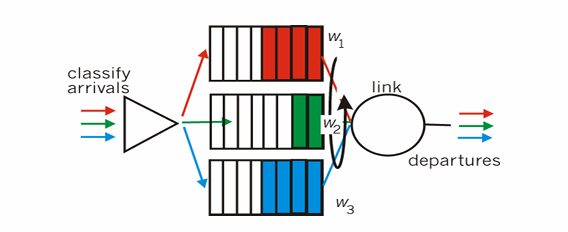
\includegraphics[width=0.76\textwidth]{router_15.png}
    \caption{%
        \textbf{Weighted Fair Queuing (WFQ) -- tre code con pesi diversi.}
        I pacchetti in arrivo vengono \textbf{classificati} e smistati in
        tre code separate, ognuna con un peso $w_1, w_2, w_3$ assegnato
        staticamente. Il \textbf{server} (il link di uscita) non scansiona
        le code in modo ciclico uniforme come nel Round Robin, ma le serve
        in modo \textbf{proporzionale ai pesi}: per ogni ciclo di
        scheduling, dalla coda $i$ viene trasmessa una quantità di dati
        proporzionale a $w_i / \sum_j w_j$.
        Le frecce oblique di diversa lunghezza indicano visivamente questa
        asimmetria: la coda con peso maggiore ``aspira'' più banda per
        unità di tempo. La garanzia è valida \emph{in media}: non si
        promette che ogni singolo pacchetto arrivi entro un certo ritardo,
        ma che nel lungo periodo ogni classe riceva esattamente la
        frazione di banda assegnata.
    }
    \label{fig:wfq}
\end{figure}

WFQ combina i vantaggi di Round Robin e Priority Scheduling:
\begin{itemize}
    \item \textbf{Nessuna starvation}: ogni classe con peso $w_i > 0$ è
          garantita di ricevere almeno la frazione $w_i / \sum_j w_j$
          della banda disponibile, indipendentemente dal carico delle
          altre classi.
    \item \textbf{Differenziazione del servizio}: assegnando pesi diversi
          si privilegiano alcune classi (VoIP, video in tempo reale)
          rispetto ad altre (bulk transfer, backup) senza mai affamarle.
    \item \textbf{Garanzie di banda minima}: utile per SLA
          (\textit{Service Level Agreement}) contrattuali -- un ISP può
          garantire a un cliente almeno $X$~Mbps dedicati anche nelle
          ore di punta.
\end{itemize}

\begin{urgentbox}{Limite fondamentale del WFQ: la garanzia vale solo
nodo per nodo}

WFQ garantisce la distribuzione della banda \textbf{all'interno di un
singolo router}. Il problema nasce appena il datagramma lascia quel
router: se il \textbf{router successivo} sul percorso non implementa
alcun meccanismo di differenziazione (o usa pesi diversi), la
classificazione ottenuta nel primo router è \emph{persa} -- il secondo
router tratta tutti i pacchetti allo stesso modo, vanificando le
garanzie precedenti.

La conseguenza pratica è immediata:

\begin{itemize}
    \item \textbf{Nella propria rete LAN / rete privata}: si
          controllano tutti i router del percorso. Si possono
          configurare gli stessi pesi WFQ su ogni nodo $\Rightarrow$
          le garanzie di banda e priorità si propagano end-to-end
          lungo tutto il percorso interno. Questo è il caso tipico
          delle reti aziendali, dei data center e delle reti degli
          operatori telefonici sulla propria infrastruttura.

    \item \textbf{Su Internet pubblico}: i datagrammi attraversano
          router di ISP diversi, sui quali non si ha alcun controllo
          né visibilità. Non si può sapere se implementano WFQ,
          Priority Scheduling o semplice FIFO. Di conseguenza
          \textbf{non è possibile garantire} banda minima, ritardo
          massimo o jitter su percorsi che attraversano Internet --
          qualsiasi garanzia di QoS si ferma al confine della propria
          rete.
\end{itemize}

\textbf{In sintesi}: WFQ risolve il problema dello scheduling
\emph{localmente}, ma la \textbf{QoS end-to-end} richiede che
\emph{ogni} router sul percorso implementi una politica coerente.
Su Internet questo non è garantito, ed è per questo che servizi
con requisiti stringenti di ritardo (VoIP, videoconferenza) vengono
tipicamente erogati su reti private o su circuiti dedicati (MPLS,
VPN) dove l'operatore controlla l'intera catena di router.
\end{urgentbox}

\begin{esempiobox}{title=Esempio pratico: Weighted Fair Queuing e garanzia di banda}
  In questo scenario, come illustrato in figura, supponiamo che il router debba gestire tre tipologie di traffico smistate in tre code separate, a ciascuna delle quali è assegnato un peso ($w$) differente:
  
  \begin{figure}[H]
      \centering
      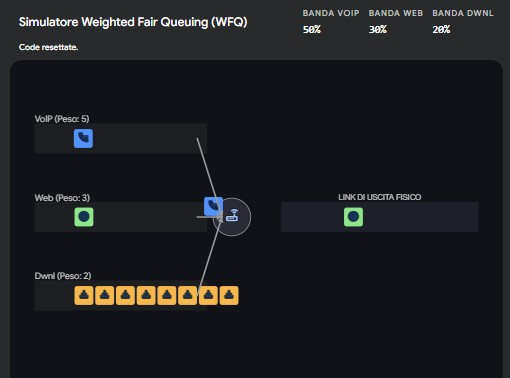
\includegraphics[width=0.6\linewidth]{WFQ.jpg}
      \caption{Simulatore di Weighted Fair Queuing (WFQ) con allocazione della banda in base ai pesi assegnati.}
      \label{fig:wfq_example}
  \end{figure}

  \begin{itemize}
      \item \textbf{VoIP:} peso $w_1 = 5$
      \item \textbf{Web:} peso $w_2 = 3$
      \item \textbf{Download (Dwnl):} peso $w_3 = 2$
  \end{itemize}

  La somma totale dei pesi è $5 + 3 + 2 = 10$. Applicando la formula del WFQ, il router calcola l'esatta frazione di banda garantita a ciascuna coda durante i momenti di congestione:
  \begin{itemize}
      \item \textbf{Banda VoIP:} $5 / 10 = \mathbf{50\%}$
      \item \textbf{Banda Web:} $3 / 10 = \mathbf{30\%}$
      \item \textbf{Banda Download:} $2 / 10 = \mathbf{20\%}$
  \end{itemize}

  \vspace{0.2cm}
  \textbf{Prevenzione della Starvation} \\
  Il link di uscita (il "server") lavora a cicli proporzionali. In ogni round di trasmissione preleverà 5 pacchetti dalla coda VoIP, 3 dalla coda Web e 2 dalla coda Download, per poi ricominciare daccapo. 
  
  Se una coda dovesse saturarsi (ad esempio, l'accumulo di pacchetti visibile nella coda Download nell'immagine), il router non si fermerà a svuotarla completamente ignorando le altre. Trasmetterà la sua quota spettante e passerà obbligatoriamente il turno alle code VoIP e Web. Questo meccanismo garantisce matematicamente che ogni tipo di traffico riceverà sempre la propria percentuale di risorse, impedendo che qualsiasi coda vada incontro a un blocco indefinito (\textit{starvation}).
\end{esempiobox}
\newpage

\subsection{Riepilogo comparativo dei 4 meccanismi di scheduling}
\begin{tcolorbox}[colback=unibolight, colframe=uniboblue,
    title=\bfseries Riepilogo dei meccanismi di scheduling,
    breakable]
\small
\renewcommand{\arraystretch}{1.5}
\begin{tabularx}{\textwidth}{p{2.2cm} X X X X}
\toprule
\textbf{Algoritmo}
    & \textbf{Equità}
    & \textbf{Differenziazione del servizio}
    & \textbf{Rischio di starvation}
    & \textbf{Complessità} \\
\midrule

\textbf{FIFO}
    & Totale: ogni pacchetto aspetta il suo turno in ordine di arrivo
    & Nessuna: tutti i pacchetti trattati allo stesso modo
    & \textcolor{okgreen}{\textbf{Assente}}: nessuna classe esiste, ogni pacchetto viene prima o poi servito
    & Minima \\

\addlinespace[3pt]
\textbf{Priority}
    & Nessuna: le classi alte dominano completamente
    & Sì: classi di priorità distinte
    & \textcolor{alertred}{\textbf{Alta}}: le classi a bassa priorità possono non essere mai servite se quelle alte non si svuotano mai (\textit{starvation} permanente)
    & Bassa \\

\addlinespace[3pt]
\textbf{Round Robin}
    & Per classe: ogni classe riceve lo stesso numero di \textit{slot} di trasmissione
    & Sì: classi distinte
    & \textcolor{okgreen}{\textbf{Assente}}: ogni classe riceve almeno uno slot per ciclo, nessuna può essere bloccata indefinitamente
    & Media \\

\addlinespace[3pt]
\textbf{WFQ}
    & Per classe: ogni classe riceve una frazione di banda proporzionale al peso $w_i$
    & Sì: pesi arbitrari $w_i$ per classe
    & \textcolor{okgreen}{\textbf{Assente}}: ogni classe con $w_i > 0$ è garantita di ricevere almeno $w_i / \sum_j w_j$ della banda disponibile
    & Alta \\

\bottomrule
\end{tabularx}
\end{tcolorbox}
\begin{collegamentobox}[title=�� Collegamento: Ritardo e Jitter]
  Il \textit{Ritardo del collegamento } e il \textit{Jitter} introdotti come indici di prestazione nel \textbf{Capitolo 1 sezione 1.4} avvengono fisicamente qui. 
  Le oscillazioni nel tempo di ricezione (Jitter) dipendono da quanto tempo i pacchetti restano "parcheggiati" nei buffer di ingresso o uscita a causa della contesa del fabric o del link.
\end{collegamentobox}

\newpage
% ============================================================
\subsection{Il percorso completo di un datagramma nel router}
% ============================================================

Riassumiamo il percorso end-to-end di un datagramma all'interno del router,
collegando tutti i componenti descritti:

\begin{enumerate}
    \item \textbf{Arrivo sul link fisico}: i bit arrivano sul link fisico
          e vengono decodificati dalla \textit{line termination} della
          porta di ingresso (\textit{livello fisico}).
    \item \textbf{Decodifica del frame}: il protocollo data-link (es.\
          Ethernet) estrae il datagramma IP rimuovendo l'header e il
          trailer del frame.
    \item \textbf{Lookup nella forwarding table}: il valore dell'indirizzo
          IP di destinazione (o altri campi in SDN) viene confrontato con
          la forwarding table locale tramite \textbf{Longest Prefix
          Matching} in TCAM -- operazione in un ciclo di clock.
    \item \textbf{Accodamento all'ingresso} (eventuale): se lo switching
          fabric è occupato, il datagramma attende nella coda della porta
          di ingresso, con rischio di HOL blocking.
    \item \textbf{Attraversamento dello switching fabric}: il datagramma
          viene trasferito dalla porta di ingresso alla porta di uscita
          selezionata tramite il meccanismo di switching (memoria, bus
          o crossbar).
    \item \textbf{Accodamento all'uscita} (eventuale): se la porta di
          uscita sta già trasmettendo, il datagramma attende in coda;
          il meccanismo di scheduling decide l'ordine di trasmissione.
    \item \textbf{Trasmissione sul link}: il protocollo data-link aggiunge
          l'header del frame e la \textit{line termination} converte i
          bit in segnali fisici per il prossimo link.
\end{enumerate}

\begin{notebox}{Cosa NON fa il router per ogni pacchetto}
Per mantenere la velocità di forwarding in nanosecondi, il data plane
\textbf{non esegue} per ogni pacchetto: 
\begin{itemize}
    \item 
aggiornamenti della routing table
(lo fa solo il routing processor, raramente)

\item  calcolo di percorsi alternativi

\item 
frammentazione IP se
non necessaria


\end{itemize}
Tutto ciò che potrebbe
rallentare il forwarding è delegato al control plane o alla sorgente.
\end{notebox}







\newpage
% ============================================================
\section{IPv4: approfondimenti ed esempi (integrano capitolo 3)  }
% ============================================================

\subsection{Il livello di rete Internet (3): componenti che interagiscono}

Il livello di rete di Internet è composto da tre componenti principali che interagiscono tra loro:

\begin{figure}[H]
\centering
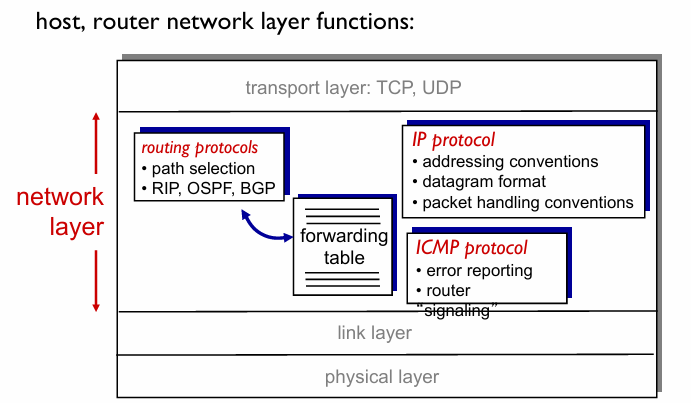
\includegraphics[width=0.7\textwidth]{router_16.png}
\caption{I componenti del livello di rete Internet}
\label{fig:internet-network-layer}
\end{figure}

\begin{itemize}
    \item \textbf{Protocolli di routing} (RIP, OSPF, BGP): selezionano i percorsi, calcolano la forwarding table.
    \item \textbf{Protocollo IP}\footnote{Vedi anche sezione 3.3.3 capitolo 3}: definisce il formato dei datagrammi, le convenzioni di indirizzamento e le regole di gestione dei pacchetti.
    \item \textbf{Protocollo ICMP}\footnote{Vedi sezione 3.3.9 capitolo 3}: segnalazione di errori e messaggi di controllo tra host e router.
\end{itemize}

\newpage
\subsection{Formato del datagramma IPv4}

Il datagramma IPv4 ha un header di \textbf{almeno 20 byte} (senza
opzioni), seguiti dai dati.

\begin{figure}[H]
\centering
\begin{tikzpicture}[scale=0.95]
    % ---- RIGA 1 ----
    \draw[thick, fill=blue!8] (0,0) rectangle (12, 0.6);
    \node[font=\small] at (0.6, 0.3) {ver};
    \node[font=\small] at (1.5, 0.3) {IHL};
    \node[font=\small] at (3.0, 0.3) {ToS/DSCP};
    \node[font=\small] at (7.5, 0.3) {Total Length (16 bit)};
    \draw (1.2,0) -- (1.2,0.6);
    \draw (1.8,0) -- (1.8,0.6);
    \draw (4.2,0) -- (4.2,0.6);
    % ---- RIGA 2 ----
    \draw[thick, fill=blue!8] (0,-0.6) rectangle (12, 0);
    \node[font=\small] at (3.5, -0.3) {Identifier (16 bit)};
    \node[font=\small] at (7, -0.3) {Flags};
    \node[font=\small] at (10.3, -0.3) {Fragment Offset (13 bit)};
    \draw (6.0,-0.6) -- (6.0,0);
    \draw (8.0,-0.6) -- (8.0,0);
    % ---- RIGA 3 ----
    \draw[thick, fill=blue!8] (0,-1.2) rectangle (12, -0.6);
    \node[font=\small] at (2, -0.9) {TTL (8 bit)};
    \node[font=\small] at (5.5, -0.9) {Protocol (8 bit)};
    \node[font=\small] at (9.5, -0.9) {Header Checksum (16 bit)};
    \draw (3.5,-1.2) -- (3.5,-0.6);
    \draw (7.0,-1.2) -- (7.0,-0.6);
    % ---- RIGA 4 ----
    \draw[thick, fill=blue!8] (0,-1.8) rectangle (12, -1.2);
    \node[font=\small] at (6, -1.5) {Source IP Address (32 bit)};
    % ---- RIGA 5 ----
    \draw[thick, fill=blue!8] (0,-2.4) rectangle (12, -1.8);
    \node[font=\small] at (6, -2.1) {Destination IP Address (32 bit)};
    % ---- OPZIONI ----
    \draw[thick, dashed, fill=blue!4] (0,-3.0) rectangle (12, -2.4);
    \node[font=\small\itshape] at (6, -2.7) {Options (variabile, opzionale)};
    % ---- DATI ----
    \draw[thick, fill=green!8] (0,-4.8) rectangle (12, -3.0);
    \node[font=\small\bfseries] at (6, -3.5) {Data (payload)};
    \node[font=\small] at (6, -4.0)
        {segmento TCP/UDP -- i dati \emph{utili} dell'applicazione};

    % ---- FRECCIA larghezza 32 bit ----
    \draw[|<->|, blue, thin] (0, 0.85) -- (12, 0.85)
        node[midway, above, font=\small\bfseries, blue]{32 bit = 4 byte per riga};

    % ---- GRAFFA header IP (20 byte = 5 righe) ----
    \draw[decorate, decoration={brace, amplitude=6pt},
          thick, alertred]
        (12.3, 0.6) -- (12.3, -2.4)
        node[midway, right=8pt, font=\small\bfseries, alertred,
             align=left] {Header IP\\20 byte\\(5 righe $\times$ 4 byte)};

    % ---- GRAFFA dati ----
    \draw[decorate, decoration={brace, amplitude=6pt},
          thick, okgreen]
        (12.3, -3.0) -- (12.3, -4.8)
        node[midway, right=8pt, font=\small\bfseries, okgreen,
             align=left] {Payload\\(variabile)};
\end{tikzpicture}
\caption{%
    \textbf{Formato del datagramma IPv4.}
    Ogni riga del diagramma rappresenta \textbf{32 bit = 4 byte}.
    L'header obbligatorio occupa \textbf{5 righe = 20 byte} (evidenziate
    in blu). Il campo \textit{Options} è opzionale e raramente usato.
    Il \textit{payload} (verde) contiene i dati utili dell'applicazione.%
}
\label{fig:ipv4-datagram}
\end{figure}

\subsubsection*{Cos'è l'overhead e perché conta}
\begin{defbox}{Overhead}
    
Il termine \textbf{overhead} indica i byte che devono essere trasmessi
\emph{in aggiunta} ai dati utili dell'applicazione, esclusivamente per
permettere al protocollo di funzionare. Non trasportano informazione
applicativa: servono alla rete per sapere dove mandare il pacchetto,
come riassemblarlo, se è corrotto, ecc.
\end{defbox}

Per una tipica connessione TCP su IPv4, l'overhead \textbf{minimo}
si accumula su due livelli:

\begin{center}
\begin{tikzpicture}[scale=0.92]
    % Pacchetto completo
    \draw[thick, fill=alertred!15] (0,0) rectangle (2.0, 0.8);
    \node[font=\small\bfseries, alertred] at (1.0, 0.4) {TCP header};
    \node[font=\tiny, alertred] at (1.0, -0.18) {20 byte};

    \draw[thick, fill=blue!15] (2.0,0) rectangle (4.0, 0.8);
    \node[font=\small\bfseries, blue] at (3.0, 0.4) {IP header};
    \node[font=\tiny, blue] at (3.0, -0.18) {20 byte};

    \draw[thick, fill=green!15] (4.0,0) rectangle (10.0, 0.8);
    \node[font=\small\bfseries, okgreen] at (7.0, 0.4)
        {Dati applicazione (payload utile)};

    % freccia overhead
    \draw[|<->|, thick, gray] (0, 1.1) -- (4.0, 1.1)
        node[midway, above, font=\small\bfseries]
        {\textbf{40 byte di overhead}};

    % freccia dati
    \draw[|<->|, thick, okgreen] (4.0, 1.1) -- (10.0, 1.1)
        node[midway, above, font=\small, okgreen]
        {dati utili};
\end{tikzpicture}
\end{center}

\vspace{0.3cm}

\[
\text{Overhead minimo} = \underbrace{20\,\text{byte}}_{\text{header TCP}}
+ \underbrace{20\,\text{byte}}_{\text{header IP}}
= \boxed{40\,\text{byte}}
\]

Questi 40 byte \textbf{devono sempre essere trasmessi} prima ancora di
inviare un singolo byte di dati utili. L'impatto pratico dipende dalla
dimensione del payload:

\begin{center}
\begin{tabular}{lrrr}
\toprule
\textbf{Scenario} & \textbf{Payload} & \textbf{Overhead} &
\textbf{Efficienza} \\
\midrule
Pacchetto massimo (MTU Ethernet) & 1460 byte & 40 byte & 97.3\% \\
Pacchetto medio & 500 byte  & 40 byte & 92.6\% \\
Risposta HTTP piccola & 100 byte & 40 byte & 71.4\% \\
ACK TCP puro (solo conferma) & \textbf{0 byte} & 40 byte &
\textbf{0\%} \\
\bottomrule
\end{tabular}
\end{center}

\begin{notebox}{Il caso peggiore: l'ACK puro}
Un segmento TCP di puro acknowledgement (nessun dato, solo conferma
di ricezione) trasporta \textbf{0 byte utili} ma occupa comunque
40 byte sulla rete -- 20 di header IP + 20 di header TCP.

\vspace{0.5cm}
L'efficienza è zero: si ``paga'' il pieno overhead senza trasportare
nulla. Questo è inevitabile: TCP deve inviare ACK per garantire
l'affidabilità, e ogni ACK deve avere il proprio header IP per essere
instradato. Nelle connessioni interattive (SSH, Telnet) questo fenomeno
è molto frequente -- ogni tasto premuto genera un pacchetto da 1 byte
di payload con 40 byte di overhead.
\end{notebox}


\subsubsection*{Descrizione dettagliata dei campi dell'header IPv4}
\vspace{1cm}
\subsubsection*{Prima riga}
\begin{itemize}

    \item \textbf{Version -- ver (4 bit)}: indica la versione del
          protocollo IP usata per costruire il datagramma. Il router
          legge questo campo \emph{prima} di qualsiasi altro per sapere
          come interpretare il resto dell'header.
          \begin{itemize}
              \item \texttt{0100} (decimale 4) $\Rightarrow$ IPv4
              \item \texttt{0110} (decimale 6) $\Rightarrow$ IPv6
          \end{itemize}
          Un router che riceve un datagramma con versione non riconosciuta
          lo scarta immediatamente.

    \item \textbf{IHL -- Internet Header Length (4 bit)}: lunghezza
          dell'header espressa in \textbf{parole da 32 bit} (non in
          byte). Necessario perché il campo \textit{Options} ha
          lunghezza variabile e il router deve sapere dove finisce
          l'header e inizia il payload.
          \begin{itemize}
              \item Valore minimo: \textbf{5} $= 5 \times 4 = 20$~byte
                    (header senza opzioni).
              \item Valore massimo: \textbf{15} $= 15 \times 4 = 60$~byte
                    (header con opzioni al massimo).
          \end{itemize}

    \item \textbf{ToS / DSCP (8 bit)}: campo originariamente chiamato
          \textit{Type of Service}, ridefinito dallo standard
          \textbf{DiffServ} come \textit{Differentiated Services Code
          Point}. 
          
          Indica la \textbf{classe di servizio} del datagramma
          e la sua priorità di forwarding nei router che implementano
          QoS. I sei bit più significativi (\textit{DSCP}) codificano
          la classe; i due bit meno significativi
          (\textit{ECN}) segnalano congestione imminente senza
          scartare pacchetti.
          \begin{notebox}{}
          In Wireshark questo campo appare quasi sempre come
          \texttt{0x00} (tutti zeri): la maggior parte delle
          applicazioni consumer non imposta alcuna priorità e lascia
          il campo a zero, affidandosi al trattamento \textit{best
          effort} standard di Internet.
          \end{notebox}

           \item \textbf{Total Length (16 bit)}: lunghezza totale del
          datagramma in byte, \textbf{header incluso}. Permette al
          destinatario di sapere quanti byte leggere dal flusso di
          dati.
          \begin{itemize}
              \item Valore minimo: 20~byte (solo header, nessun dato).
              \item Valore massimo: $2^{16} - 1 = 65\,535$~byte.
              \item Nella pratica il limite è l'MTU del link (1500~byte
                    per Ethernet): datagrammi più grandi vengono
                    frammentati.
          \end{itemize}


\newpage
\subsubsection*{Seconda riga}
   

    \item \textbf{Identifier (16 bit)}: numero intero assegnato dal
          mittente al momento della creazione del datagramma. Tutti i
          \textbf{frammenti} prodotti dalla frammentazione di un
          datagramma originale portano lo \textbf{stesso Identifier},
          così il destinatario finale può raggruppare i frammenti
          appartenenti allo stesso datagramma e riassemblarli
          nell'ordine corretto.
    \item \textbf{Flags (3 bit)}: tre bit di controllo per la
      frammentazione. I bit sono indipendenti tra loro --
      ognuno ha il proprio significato:
      \begin{itemize}
          \item \textbf{bit 0 -- riservato}: sempre 0, non usato.

          \item \textbf{bit 1 -- DF (\textit{Don't Fragment})}:
                controlla se il datagramma \emph{può} essere
                frammentato.
                \begin{itemize}
                    \item \textbf{DF = 0}: la frammentazione è
                          \emph{permessa} -- il router può
                          spezzare il datagramma se necessario.
                    \item \textbf{DF = 1}: la frammentazione è
                          \emph{vietata} -- se il datagramma è
                          troppo grande per il link, il router
                          lo \textbf{scarta} e invia un messaggio
                          ICMP ``Fragmentation Needed'' al
                          mittente, che dovrà ritrasmettere con
                          un datagramma più piccolo. Questo
                          meccanismo si chiama
                          \textbf{Path MTU Discovery}.
                \end{itemize}

          \item \textbf{bit 2 -- MF (\textit{More Fragments})}:
                segnala se esistono altri frammenti dopo questo.
                \begin{itemize}
                    \item \textbf{MF = 1}: questo \emph{non} è
                          l'ultimo frammento -- ne seguono altri.
                    \item \textbf{MF = 0}: questo è l'ultimo
                          frammento (oppure il datagramma non
                          è stato frammentato affatto).
                \end{itemize}
      \end{itemize}

\begin{esempiobox}{Come leggere i Flags insieme}
Un datagramma \textbf{non frammentato} ha sempre:
\texttt{DF=0, MF=0, offset=0}.

Quando un router frammenta un datagramma in 3 pezzi:
\begin{center}
\begin{tabular}{lccc}
\toprule
\textbf{Frammento} & \textbf{DF} & \textbf{MF} &
\textbf{Offset} \\
\midrule
1° (primo)  & 0 & \textbf{1} & 0   \\
2° (medio)  & 0 & \textbf{1} & 185 \\
3° (ultimo) & 0 & \textbf{0} & 370 \\
\bottomrule
\end{tabular}
\end{center}
Il destinatario riconosce l'ultimo frammento dal fatto che
ha \texttt{MF=0} \emph{con} un offset $> 0$.
Un datagramma con \texttt{MF=0} e \texttt{offset=0}
non è mai stato frammentato.
\end{esempiobox}

    \item \textbf{Fragment Offset (13 bit)}: posizione dei dati
          contenuti in questo frammento rispetto all'inizio del
          datagramma originale, espressa in \textbf{unità di 8 byte}.
          Il primo frammento ha offset = 0. Permette al destinatario
          di riassemblare i frammenti nell'ordine corretto anche se
          arrivano fuori sequenza.
          \[
              \text{Offset reale (byte)} = \text{Fragment Offset}
              \times 8
          \]

\newpage
\subsubsection*{Terza riga}
    \item \textbf{TTL -- Time To Live (8 bit)}: contatore decrementato
          di 1 da \textbf{ogni router} che inoltra il datagramma.
          Quando raggiunge 0, il datagramma viene \textbf{scartato} e
          il router invia un messaggio ICMP ``Time Exceeded'' al
          mittente.
          
          Scopo: prevenire che datagrammi ``vaganti'' per
          loop di routing circolino indefinitamente occupando banda.
          Il valore iniziale tipico è 64 (Linux) o 128 (Windows).
          Il comando \texttt{traceroute} sfrutta deliberatamente
          questo meccanismo: invia datagrammi con TTL = 1, 2, 3,
          \ldots\ e raccoglie i messaggi ICMP per ricostruire il
          percorso.

    \item \textbf{Protocol (8 bit)}: identifica il protocollo del
          \textbf{livello di trasporto} (\textit{upper layer protocol})
          incapsulato nel payload. Svolge la funzione di
          \textit{demultiplexing} al livello di rete: il destinatario
          usa questo campo per consegnare il payload al modulo
          corretto.
          \begin{center}
          \begin{tabular}{ll}
          \toprule
          \textbf{Valore} & \textbf{Protocollo} \\
          \midrule
          1  & ICMP \\
          6  & TCP  \\
          17 & UDP  \\
          89 & OSPF \\
          \bottomrule
          \end{tabular}
          \end{center}

    \item \textbf{Header Checksum (16 bit)}: checksum calcolato
          \textbf{solo sull'header IP} (non sui dati). Permette al
          router di rilevare errori di trasmissione nell'header.
          Deve essere \textbf{ricalcolato ad ogni hop} perché il TTL
          cambia a ogni router -- questo è uno dei motivi per cui
          IPv6 ha eliminato questo campo (overhead inutile sui link
          moderni molto affidabili).

\vspace{0.5cm}
\subsubsection*{Quarta riga}
    \item \textbf{Source Address (32 bit)}: indirizzo IP
          dell'interfaccia mittente. Usato dal destinatario per
          inviare le risposte e dai firewall per applicare regole di
          filtraggio. Può essere falsificato (\textit{IP spoofing})
          poiché IP non autentica la sorgente.

\vspace{0.5cm}
\subsubsection*{Quinta riga}
    \item \textbf{Destination Address (32 bit)}: indirizzo IP
          dell'interfaccia destinataria. È il campo usato da ogni
          router per il \textbf{longest prefix matching} nella
          forwarding table.

    \item \textbf{Options (variabile, 0--40 byte)}: campo opzionale,
          raramente usato nella pratica ma importante storicamente.
          Le opzioni principali sono:
          \begin{itemize}
              \item \textbf{Timestamp}: ogni router aggiunge il
                    proprio indirizzo IP e il tempo di transito.
                    Utile per misurare la latenza lungo il percorso.
              \item \textbf{Record Route}: ogni router aggiunge il
                    proprio indirizzo IP alla lista. Il destinatario
                    riceve la \textbf{lista completa dei router
                    attraversati} -- utile per diagnostica e
                    troubleshooting di rete, simile a traceroute ma
                    implementato direttamente nell'header IP.
             
          \end{itemize}
          La presenza di opzioni rallenta il processing nei router
          perché l'hardware non può assumere header a lunghezza fissa
          -- uno dei motivi principali per cui IPv6 le ha spostate
          fuori dall'header principale.

\end{itemize}

\begin{collegamentobox}[title=�� Focus: IPv4 (Cap. 3) vs Datagramma IPv4 (Cap. 5)]
  Il focus passa dalla logica all'implementazione fisica:
  \begin{itemize}
      \item \textbf{Capitolo 3 (Indirizzamento) sezione 3.3.4 :} È l'\textit{etichetta con il nome}. Si concentra su \textbf{chi} sono i nodi (IP source e destination ). Tratta l'indirizzo a 32 bit come identificatore puro, analizzando la divisione logica tra \textit{Network ID} e \textit{Host ID}, le classi (A, B, C) e il subnetting.
      \item \textbf{Capitolo 5 (Formato Datagramma):} È il \textit{pacco postale completo}. Si concentra su \textbf{come} viaggiano i dati sui cavi. Analizza l'intera "scatola" (l'Header IP da minimo 20 byte), l'overhead di rete e i campi di servizio essenziali ai router, come il TTL, il Checksum e le istruzioni per la \textit{frammentazione}. 
      
      Nel datagramma è contenuto l'identificatore mittente e destinatario (trattati nella sezione \textbf{3.3.4}) come abbiamo visto in questa sezione.
  \end{itemize}
\end{collegamentobox}


\subsection{Frammentazione e Riassemblaggio (solo IPv4)}

\begin{figure}[H]
    \centering
    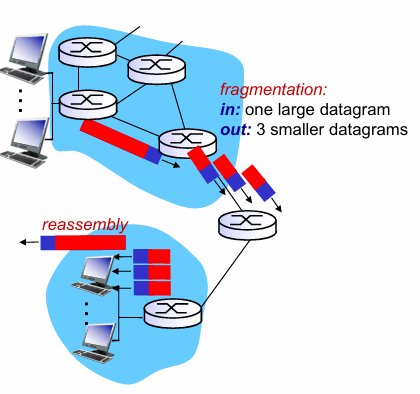
\includegraphics[width=0.4\linewidth]{router_17.png}
    \caption{router si scambiano pacchetti con header e payload. Arrivato ad un certo router la se la dimensione del pacchetto è troppo grande e viene frammentato}
    \label{fig:placeholder}
\end{figure}
\begin{defbox}{MTU -- Maximum Transmission Unit}
Ogni link ha un \textbf{MTU} (\textit{Maximum Transfer Unit}): la dimensione massima del frame a livello data link. Tecnologie diverse hanno MTU diversi (Ethernet: 1500 byte, WiFi: variabile, ecc.).
\end{defbox}

Se un datagramma IP è più grande dell'MTU del link che deve attraversare, il router lo \textbf{frammenta}: lo divide in datagrammi più piccoli (frammenti), ciascuno con il proprio header IP. I frammenti vengono riassemblati \textbf{solo all'host destinazione finale} (non ai router intermedi).

I campi usati per il riassemblaggio sono:
\begin{itemize}
\item \textbf{Length:} lunghezza del frammento
    \item \textbf{Identifier}: tutti i frammenti dello stesso datagramma originale hanno lo stesso identifier.
    \item \textbf{Fragment Offset}: posizione del frammento nel datagramma originale (in unità di 8 byte).Indice che mi dice da quale byte parte questo pacchetto nel pacchetto iniziale
    \item \textbf{More Fragments (MF) flag}: 1 per tutti i frammenti tranne l'ultimo.
\end{itemize}

\newpage
\begin{esempiobox}{Esempio di frammentazione}
Un datagramma (ID = x) di 4000 byte deve attraversare un link con MTU = 1500 byte.
\begin{itemize}
    \item Ogni frammento può portare al massimo $1500 - 20 = 1480$ byte di dati.
    \item Frammento 1; dati byte 0--1479 (20 byte sono la dim dell'header):
    
    \begin{center}
        {length=1500 | offset=0 (primo byte del payload) | MF=1 (more fragment)| ID=x}
    \end{center} 
    
    \item Frammento 2; dati byte 1480--2959:
    \begin{center}
        
    length=1500 | offset=185 ($=1480/8$) | MF=1 | ID=x
    \end{center}
    
    \item Frammento 3; dati byte 2960--3979 (1040):
    \begin{center}
        
    length=1020 | offset=370 ($=2960/8$) | MF=0 | ID=x
    \end{center}
\end{itemize}

\begin{center}
\begin{tikzpicture}[scale=0.9]
% Datagramma originale
\draw[thick, fill=blue!10] (0,2) rectangle (8,2.8);
\node[font=\small] at (1, 2.4) {Hdr};
\draw (1.5,2) -- (1.5,2.8);
\node[font=\small] at (4.75, 2.4) {Dati: 3980 byte};
\node[above, font=\small] at (4, 2.8) {Datagramma originale: 4000 byte, ID=x, offset=0, MF=0};

\draw[->, thick] (4, 2) -- (4, 1.5);
\node[font=\small] at (4, 1.3) {MTU = 1500 byte};
\draw[->, thick] (4, 1.1) -- (4, 0.7);

% Tre frammenti
\foreach \x/\label/\off/\mf/\col in {0/F1/0/1/red!15, 3.2/F2/185/1/green!15, 6.4/F3/370/0/orange!15}{
    \draw[thick, fill=\col] (\x, 0) rectangle (\x+2.8, 0.6);
    \node[font=\tiny] at (\x+0.3, 0.3) {H};
    \draw (\x+0.6, 0) -- (\x+0.6, 0.6);
    \node[font=\tiny] at (\x+1.7, 0.3) {Dati};
    \node[below, font=\tiny, align=center] at (\x+1.4, 0) {\label: off=\off, MF=\mf};
}
\end{tikzpicture}
\end{center}
\end{esempiobox}

\begin{notebox}{IPv6 e frammentazione}
IPv6 \textbf{non supporta} la frammentazione nei router: se un datagramma IPv6 è troppo grande per il link, il router lo scarta e invia un messaggio ICMPv6 ``Packet Too Big'' all'host sorgente, che deve ridurre la dimensione dei pacchetti. Questo semplifica notevolmente il lavoro dei router.
\end{notebox}






\newpage
% ============================================================
\subsection{DOMANDE: indirizzamento IPv4 (domande pratiche)}

gli esercizi a seguire faranno riferimento a questa figura:
\begin{figure}[H]
    \centering
    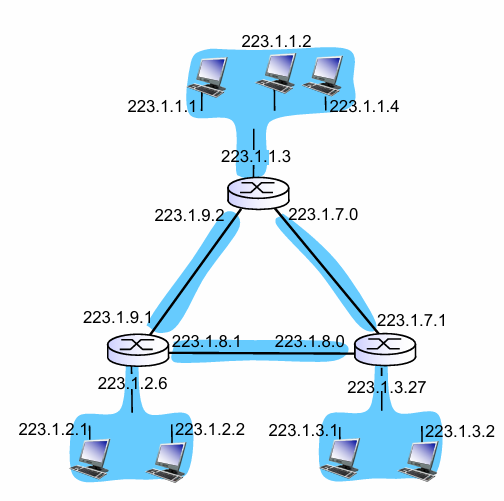
\includegraphics[width=0.5\linewidth]{router_20.png}
    \caption{}
    \label{fig:esemp}
\end{figure}

% ============================================================
\paragraph{1. Aggregare  6 subnet in una sola -- è davvero
possibile?}
% ============================================================

Le nostre 6 subnet hanno terzo ottetto
$\{1, 2, 3, 7, 8, 9\}$. Scriviamo ogni valore in binario
per trovare i blocchi aggregabili:
\textbf{
[Per unire due sottoreti /24 (dove i primi 24 bit sono fissi) in una singola sottorete /23 (dove i primi 23 bit sono fissi), i primi 23 bit dei loro indirizzi devono essere identici.]}

\begin{center}
\begin{tabular}{rlll}
\toprule
\textbf{Subnet /24} & \textbf{Terzo ottetto in binario}
    & \textbf{7 bit alti} & \textbf{Accoppiabile con} \\
\midrule
\texttt{223.1.\textbf{1}.0}
    & \texttt{0000 000\textcolor{alertred}{1}}
    & \texttt{0000 000}
    & nessuna (1 è sola nel suo /23) \\
\texttt{223.1.\textbf{2}.0}
    & \texttt{0000 001\textcolor{alertred}{0}}
    & \texttt{0000 001}
    & \texttt{.3} (stessi 7 bit) \\
\texttt{223.1.\textbf{3}.0}
    & \texttt{0000 001\textcolor{alertred}{1}}
    & \texttt{0000 001}
    & \texttt{.2} (stessi 7 bit) \\
\texttt{223.1.\textbf{7}.0}
    & \texttt{0000 011\textcolor{alertred}{1}}
    & \texttt{0000 011}
    & nessuna (7 è sola nel suo /23) \\
\texttt{223.1.\textbf{8}.0}
    & \texttt{0000 100\textcolor{alertred}{0}}
    & \texttt{0000 100}
    & \texttt{.9} (stessi 7 bit) \\
\texttt{223.1.\textbf{9}.0}
    & \texttt{0000 100\textcolor{alertred}{1}}
    & \texttt{0000 100}
    & \texttt{.8} (stessi 7 bit) \\
\bottomrule
\end{tabular}
\end{center}

\noindent Risultato: riusciamo ad aggregare solo due coppie.
Il minimo numero di prefissi da annunciare è \textbf{4}:

\begin{center}
\begin{tabular}{lll}
\toprule
\textbf{Prefisso annunciato} & \textbf{Copre} &
\textbf{Spreco} \\
\midrule
\texttt{223.1.2.0/23} & \texttt{.2} e \texttt{.3} & nessuno \\
\texttt{223.1.8.0/23} & \texttt{.8} e \texttt{.9} & nessuno \\
\texttt{223.1.1.0/24} & solo \texttt{.1} & nessuno \\
\texttt{223.1.7.0/24} & solo \texttt{.7} & nessuno \\
\bottomrule
\end{tabular}
\end{center}

\begin{urgentbox}{Perché non si può fare meglio?}
Le subnet \texttt{.1, .7} sono \textbf{isolate}: ognuna ha
7 bit alti unici, nessun'altra subnet condivide quegli stessi
7 bit. Non esiste alcun \texttt{/23} che le accoppi senza
includere subnet che non possediamo.

\textbf{Morale pratica}: se in fase di progetto avessimo
scelto subnet contigue e allineate -- es.\
$\{2,3,4,5,6,7\}$ -- avremmo potuto aggregare tutto in
\texttt{223.1.2.0/22} (copre .2,.3,.4,.5) +
\texttt{223.1.6.0/23} (copre .6,.7) = \textbf{2 soli
annunci}. Oppure scegliendo $\{0,1,2,3,4,5,6,7\}$
un unico \texttt{223.1.0.0/21}.
Questo è il motivo per cui negli appunti del Capitolo~3
(\textbf{\,3.3.5 -- Sottoreti}) si sottolinea che
la pianificazione gerarchica degli indirizzi deve
avvenire \emph{fin dall'inizio}: riassegnare
indirizzi in seguito è costoso e complesso.
\end{urgentbox}

% ============================================================
\paragraph{2. Quale default gateway per collegarsi ad Internet?}
% ===========================================================

\vspace{0.5cm}
 Consideriamo un host nella subnet
\texttt{223.1.9.0/24} con indirizzo \texttt{223.1.9.5}.
Vuole raggiungere un server su Internet (es.\
\texttt{8.8.8.8}).

\textbf{Passo 1 -- L'host capisce che la destinazione è
fuori dalla propria subnet}:

\[
    \texttt{8.8.8.8} \;\text{ AND }\;
    \underbrace{\texttt{255.255.255.0}}_{\text{subnet mask /24}}
    \;=\; \texttt{8.8.8.0}
    \;\neq\; \texttt{223.1.9.0}
    \quad \Rightarrow \quad
    \text{destinazione esterna}
\]

L'host non può consegnare il pacchetto direttamente:
deve passarlo al \textbf{default gateway} --
il router che ha un'interfaccia \emph{nella stessa subnet}
\texttt{223.1.9.x} dell'host.

\vspace{0.5cm}
\textbf{Passo 2 -- Quale indirizzo ha il default gateway?}

Nella figura \ref{fig:esemp} i due router hanno
interfacce \texttt{223.1.9.1} e \texttt{223.1.9.2}
su questa subnet. L'host sceglie \emph{uno} dei due,
tipicamente il \texttt{.1} oppure il \texttt{.254}
(ultimo indirizzo disponibile per convenzione).

\begin{notebox}{Default gateway e DHCP --
\,3.3.2, \,3.3.12, \,3.5.8 Capitolo~3}

Come descritto nell'\textbf{Algoritmo~1}
(\,3.3.2 appunti), la logica del router è:
\begin{enumerate}
    \item Il pacchetto arriva al default gateway
          \texttt{223.1.9.1}.
    \item Il router controlla la propria tabella di
          forwarding: conosce la rete destinazione?
    \item Se sì: lo instrada direttamente.
          Se no: lo passa al \textbf{default router}
          (il router di livello superiore verso Internet).
\end{enumerate}

Nella pratica domestica e aziendale questo parametro
non viene configurato manualmente: è il
\textbf{DHCP} \footnote{(\,3.3.12 e \,3.5.8 capitolo 3)}
che lo comunica automaticamente all'host insieme
all'indirizzo IP, alla subnet mask e al DNS server.
\end{notebox}

\newpage
% ============================================================
\paragraph{3. Due router, due ISP diversi
(\textit{multi-homing}).}
% ============================================================

\begin{center}
\begin{tikzpicture}[
    box/.style={rectangle, draw, rounded corners=4pt,
                fill=unibolight, minimum width=2.6cm,
                minimum height=0.8cm, font=\small,
                align=center},
    isp/.style={rectangle, draw, rounded corners=4pt,
                fill=okgreen!20, minimum width=2.2cm,
                minimum height=0.8cm, font=\small,
                align=center},
    cloud/.style={rectangle, draw, rounded corners=4pt,
                  fill=blue!10, minimum width=1.8cm,
                  minimum height=0.8cm, font=\small,
                  align=center},
    arr/.style={->, thick}
]
    \node[box] (lan) at (0,0)
        {Rete interna\\{\tiny 223.1.x.x}};
    \node[box] (ra) at (3.5, 1.0)
        {Router A\\{\tiny IP pub: \texttt{85.10.1.1}}};
    \node[box] (rb) at (3.5,-1.0)
        {Router B\\{\tiny IP pub: \texttt{91.20.2.1}}};
    \node[isp] (i1) at (7.0, 1.0) {ISP 1};
    \node[isp] (i2) at (7.0,-1.0) {ISP 2};
    \node[cloud] (inet) at (10.0, 0) {Internet};

    \draw[arr] (lan) -- (ra);
    \draw[arr] (lan) -- (rb);
    \draw[arr] (ra)  -- (i1);
    \draw[arr] (rb)  -- (i2);
    \draw[arr] (i1)  -- (inet);
    \draw[arr] (i2)  -- (inet);
\end{tikzpicture}
\end{center}

I due router hanno ognuno un \textbf{proprio indirizzo
pubblico assegnato da ISP diversi}:
\begin{itemize}
    \item Router~A riceve \texttt{85.10.1.1} da ISP~1.
    \item Router~B riceve \texttt{91.20.2.1} da ISP~2.
\end{itemize}

I due indirizzi appartengono a blocchi di proprietà di
operatori distinti: sono completamente indipendenti.

\begin{itemize}
    \item \textbf{Ridondanza}: se ISP~1 cade, tutto
          il traffico viene reindirizzato via Router~B --
          ISP~2. La rete rimane raggiungibile.
    \item \textbf{Indipendenza contrattuale}: si
          negoziano SLA diverse con due fornitori,
          scegliendo quello più conveniente per
          tipologia di traffico.
    \item \textbf{Svantaggio}: costo doppio (due
          contratti), configurazione BGP più complessa.
\end{itemize}

% ============================================================
\paragraph{4. Due indirizzi pubblici dallo stesso ISP --
stesso router di confine.}
% ============================================================

\begin{center}
\begin{tikzpicture}[
    box/.style={rectangle, draw, rounded corners=4pt,
                fill=unibolight, minimum width=2.8cm,
                minimum height=1.1cm, font=\small,
                align=center},
    isp/.style={rectangle, draw, rounded corners=4pt,
                fill=okgreen!20, minimum width=2.2cm,
                minimum height=0.8cm, font=\small,
                align=center},
    cloud/.style={rectangle, draw, rounded corners=4pt,
                  fill=blue!10, minimum width=1.8cm,
                  minimum height=0.8cm, font=\small,
                  align=center},
    arr/.style={->, thick}
]
    \node[box] (lan) at (0,0)
        {Rete interna\\{\tiny 192.168.1.x}\\
         {\tiny (indirizzi privati)}};
    \node[box] (r) at (4.0,0)
        {Router unico\\
         {\tiny WAN1: \texttt{85.10.1.1}}\\
         {\tiny WAN2: \texttt{85.10.1.2}}};
    \node[isp] (isp) at (7.8,0) {ISP unico};
    \node[cloud] (inet) at (10.8,0) {Internet};

    \draw[arr] (lan) -- (r)
        node[midway, above, font=\tiny]{NAT};
    \draw[arr, bend left=20]  (r) to
        node[above, font=\tiny]{WAN1} (isp);
    \draw[arr, bend right=20] (r) to
        node[below, font=\tiny]{WAN2} (isp);
    \draw[arr] (isp) -- (inet);
\end{tikzpicture}
\end{center}

Un \textbf{unico router di confine} ha due interfacce
WAN fisiche collegate allo stesso ISP. L'ISP assegna
\textbf{due indirizzi pubblici distinti} -- uno per
interfaccia -- allo stesso router.

La rete interna usa \textbf{indirizzi privati}
(\texttt{192.168.x.x}): il router applica il \textbf{NAT}
\footnote{(vedi sezione \textbf{\,3.3.14} 
appunti del Capitolo~3)} per tradurli verso uno dei
due IP pubblici prima di uscire su Internet.

\begin{center}
\begin{tabular}{lll}
\toprule
& \textbf{Multi-homing (caso 3)}
& \textbf{Stesso ISP (caso 4)} \\
\midrule
\textbf{Router}    & Due router distinti
                   & Un solo router, due WAN \\
\textbf{ISP}       & Due ISP diversi
                   & Un solo ISP \\
\textbf{Ridondanza}& Alta (ISP indipendenti)
                   & Bassa (se l'ISP cade, tutto cade) \\
\textbf{Banda}     & Separata per uplink
                   & Aggregabile (\textit{bonding}) \\
\textbf{Costo}     & Doppio contratto
                   & Contratto singolo \\
\textbf{Indirizzi} & Blocchi di ISP diversi
                   & Blocco unico dell'ISP \\
\bottomrule
\end{tabular}
\end{center}







\newpage

% ============================================================
\subsection{ESEMPIO: Come un host ottiene un indirizzo IP: DHCP(esempio reale)}
% ============================================================

Come discusso nel Capitolo~3 \footnote{(Sezione 3.3.12 (e poco nella 3.5.8)-- Assegnazione degli
indirizzi IP)}, esistono due modalità di assegnazione: 
\begin{itemize}
    \item 
\textbf{statica}
(l'amministratore associa manualmente un indirizzo IP al MAC
dell'interfaccia, associazione permanente)
\item   \textbf{dinamica via DHCP}
(la più diffusa)
\end{itemize} 

Qui riporto un esempio reale sulla base di quanto studiato nel capitolo 3

\begin{esempiobox}[title=Incapsulamento DHCP (DORA) e collegamento con ARP]

Le due figure mostrano il meccanismo di incapsulamento DHCP visto dal punto di vista dello stack protocollare, in un esempio reale con un laptop, uno switch e un router con server DHCP integrato (indirizzo \texttt{168.1.1.1}).

\medskip
\textbf{1. La richiesta DHCP sale e scende lo stack}

Nella fase di \textbf{DHCP REQUEST}, il messaggio attraversa i vari livelli di rete per raggiungere il server:
\begin{itemize}
    \item \textbf{Lato laptop (freccia rossa verso il basso):} il messaggio applicativo DHCP viene progressivamente incapsulato scendendo lo stack.
    
    - Prima in un segmento \textbf{UDP}  (src: porta 68, dst: porta 67), 
    
    - poi in un datagramma \textbf{IP} (src: \texttt{0.0.0.0}, dst: \texttt{255.255.255.255}  -- broadcast), 
    
    - poi in un frame \textbf{Ethernet} (src MAC: MAC mittente, dst MAC: \texttt{FF:FF:FF:FF:FF:FF}).

    
    Infine, viene convertito in segnali fisici dal livello \textbf{Phy} e trasmesso sul cavo verso lo switch.
    \item \textbf{Lo switch:} opera solo al livello 2 (MAC/LLC). Legge il MAC di destinazione di broadcast e inonda (flooding) il frame su tutte le porte.
    \item \textbf{Lato router (freccia rossa verso l'alto):} il router riceve il frame fisico e risale lo stack decapsulando ogni livello: Phy $\to$ Eth $\to$ IP $\to$ UDP $\to$ DHCP. Solo a questo punto il software DHCP del router può leggere la richiesta.
\end{itemize}

\begin{figure}[H]
    \centering
    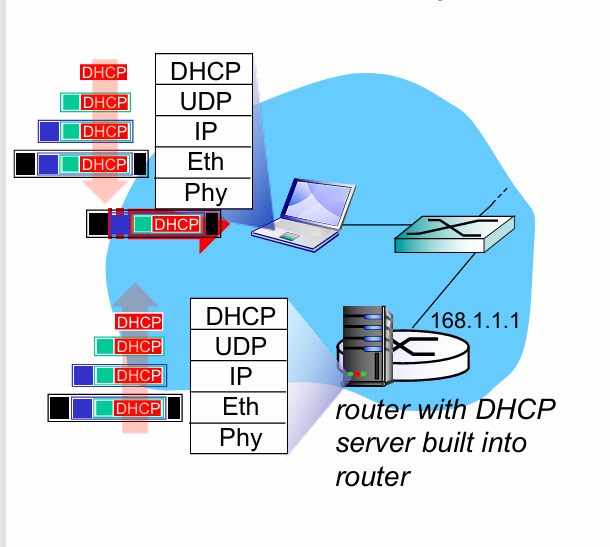
\includegraphics[width=0.5\textwidth]{router_26.png}
    \caption{\textbf{DHCP REQUEST:} incapsulamento lato client e decapsulamento lato server.}
    \label{fig:dhcp_encap_request}
\end{figure}

\medskip
\textbf{2. La risposta DHCP ACK torna al client}

Una volta elaborata la richiesta, il server formula la risposta (\textbf{DHCP ACK}) contenente l'indirizzo IP assegnato, la subnet mask, il default gateway e il DNS.
\begin{itemize}
    \item \textbf{Lato router (freccia rossa verso il basso):} scendendo lo stack, il messaggio viene:
    
    - incapsulato in \textbf{UDP} (src: porta 67, dst: porta 68),
    
    - poi in \textbf{IP} (src: \texttt{168.1.1.1}, dst: \texttt{255.255.255.255} -- ancora broadcast, poiché il client non ha ancora confermato l'IP), 
    
     - poi in \textbf{Ethernet} e trasmesso fisicamente.
    \item \textbf{Lato laptop (freccia rossa verso l'alto):} il laptop riceve il frame, risale lo stack estraendo l'ACK. Da questo momento la configurazione di rete dell'host è completa e funzionante (sempre se accetta l'oferta).
\end{itemize}

\begin{figure}[H]
    \centering
    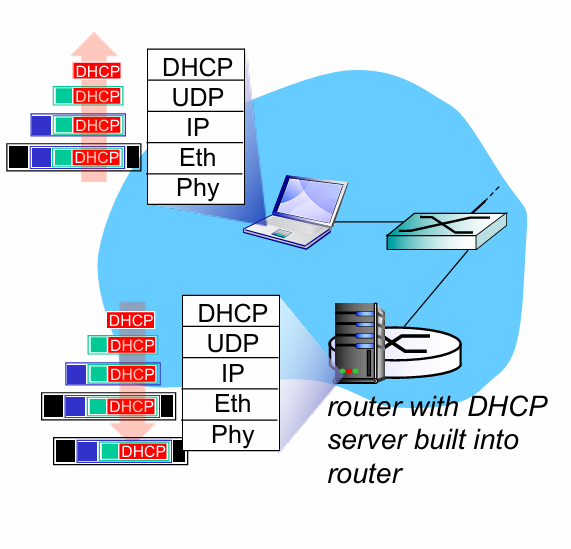
\includegraphics[width=0.62\textwidth]{router_27.png}
    \caption{\textbf{DHCP ACK:} il server formula la risposta e la invia al client.}
    \label{fig:dhcp_encap_ack}
\end{figure}

\medskip
\textbf{Perché tutti i messaggi DHCP usano il broadcast?}

\begin{center}
\begin{tabular}{lll}
\toprule
\textbf{Messaggio} & \textbf{IP sorgente} & \textbf{IP destinazione} \\
\midrule
Discover & \texttt{0.0.0.0}     & \texttt{255.255.255.255} \\
Offer    & \texttt{168.1.1.1}   & \texttt{255.255.255.255} \\
Request  & \texttt{0.0.0.0}     & \texttt{255.255.255.255} \\
ACK      & \texttt{168.1.1.1}   & \texttt{255.255.255.255} \\
\bottomrule
\end{tabular}
\end{center}

Il client usa \texttt{0.0.0.0} come sorgente perché non ha ancora un IP valido, e usa il broadcast \texttt{255.255.255.255} come destinazione perché non conosce l'indirizzo del server. Il server risponde ancora in broadcast perché il client, pur avendo ricevuto un'offerta, non ha ancora un IP \emph{confermato} e configurato con cui ricevere un normale pacchetto unicast.

\newpage
\textbf{Dopo DHCP entra in gioco ARP}

Una volta ottenuto l'indirizzo IP via DHCP, ogni volta che l'host vuole comunicare con un dispositivo della stessa subnet, deve risolvere l'IP nel MAC corrispondente tramite \textbf{ARP}\footnote{Vedi capitolo 3 sezione 3.3.11}. La logica è la seguente:

$$
    \underbrace{\texttt{168.1.1.x}}_{\text{IP -- Livello Rete (3)}}
    \;\xrightarrow{\;\text{ARP}\;}
    \underbrace{\texttt{AA:BB:CC:DD:EE:FF}}_{\text{MAC -- Livello Ethernet (2)}}
$$

ARP invia un broadcast \textit{("Chi ha questo IP? Dimmi il tuo MAC")}; solo il destinatario risponde in unicast con il proprio MAC. L'host aggiorna così la sua cache ARP e può finalmente costruire il frame Ethernet corretto.

\begin{center}
\begin{tabular}{lll}
\toprule
\textbf{Protocollo} & \textbf{Domanda a cui risponde} & \textbf{Risultato} \\
\midrule
DHCP & Chi sono sulla rete? & IP, mask, gateway, DNS \\
ARP  & Dove si trova fisicamente? & IP $\to$ MAC per il frame Ethernet \\
\bottomrule
\end{tabular}
\end{center}

I due protocolli operano in sequenza obbligata: senza DHCP l'host non ha un IP e non può fare ARP; senza ARP l'host ha un IP, ma non riesce a consegnare fisicamente nessun frame sulla LAN.

\end{esempiobox}





\newpage


% ============================================================
\newpage
\subsection{ESEMPIO: Aggregazione gerarchica degli indirizzi tramite NAT}
% ============================================================

NAT permette di \textbf{aggregare} più prefissi contigui in un unico
prefisso più corto, riducendo drasticamente la dimensione delle routing
table su Internet -- un beneficio fondamentale per la scalabilità.

\begin{figure}[H]
    \centering
    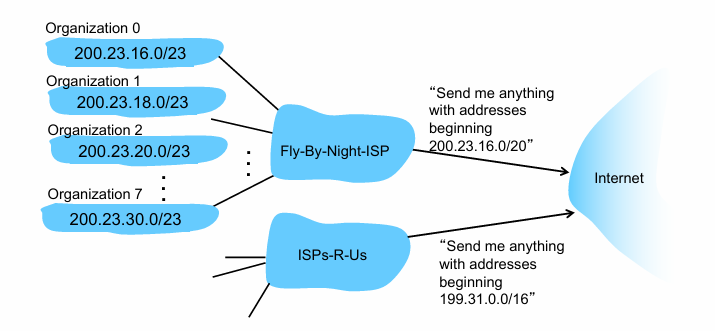
\includegraphics[width=0.85\textwidth]{route_22.png}
    \caption{%
        \textbf{Aggregazione gerarchica -- route aggregation.}
        L'ISP \textit{Fly-By-Night} possiede il blocco
        \texttt{200.23.16.0/20} (4096 indirizzi) e lo suddivide tra
        8 organizzazioni, assegnando a ciascuna un blocco \texttt{/23}
        (512 indirizzi). Verso il resto di Internet, Fly-By-Night annuncia
        \textbf{un solo prefisso aggregato} \texttt{200.23.16.0/20}
        invece di 8 prefissi separati: i router di Internet non devono
        sapere nulla della struttura interna dell'ISP.
        L'ISP \textit{ISPs-R-Us} annuncia \texttt{199.31.0.0/16}: blocco
        completamente separato, nessuna sovrapposizione.%
    }
    \label{fig:route_aggregation}
\end{figure}

\begin{figure}[H]
    \centering
    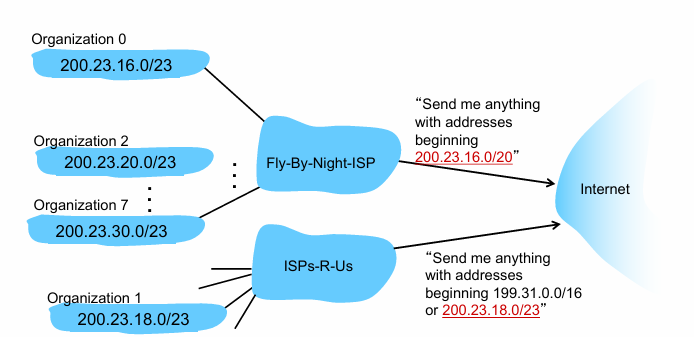
\includegraphics[width=0.85\textwidth]{route_23}
    
    \vspace{0.3cm} % Spazio tra immagine e tabella
    
    \begin{tabular}{lll}
    \toprule
    \textbf{Chi annuncia} & \textbf{Prefisso} & \textbf{Copre} \\
    \midrule
    Fly-By-Night & \texttt{200.23.16.0/\textbf{20}} & tutte le 8 org. \\
    ISPs-R-Us    & \texttt{199.31.0.0/16}           & i propri clienti \\
    ISPs-R-Us    & \texttt{200.23.18.0/\textbf{23}} & solo l'Org. 1 \\
    \bottomrule
    \end{tabular}

    \caption{\textbf{Route più specifica -- override dell'aggregazione.} Scenario di migrazione dell'Organizzazione 1 da Fly-By-Night a ISPs-R-Us. Per il \textbf{Longest Prefix Matching}, il traffico verso \texttt{200.23.18.x} viene instradato verso il prefisso \texttt{/23} (più specifico).}
    \label{fig:route_aggregation_specific}
\end{figure}



\newpage
% ============================================================
\subsection{Formato del datagramma e richiami di tunneling }
% ============================================================

\subsubsection{Motivazione}

Come introdotto nel Capitolo~3 (Sezione 3.3.13 -- IPv6 e
Tunnelling IPv4/IPv6),

IPv6 nasce dalla crescita esponenziale
dei dispositivi connessi che ha reso insufficiente lo spazio
di $2^{32} \approx 4.3$ miliardi di indirizzi IPv4.
Motivazioni aggiuntive:
\begin{itemize}
    \item Header di \textbf{formato fisso} che velocizza
          l'elaborazione dei router -- non è più necessario
          ricalcolare il checksum ad ogni hop.
    \item Modifiche all'header per facilitare il \textbf{QoS}
          (campo \textit{flow label}).
    \item Spazio di indirizzi a \textbf{128~bit} $= 2^{128}$
          indirizzi (praticamente illimitato).
    \item \textbf{Nessuna frammentazione} nei router: se un
          datagramma è troppo grande, il router lo scarta e
          invia ICMPv6 ``Packet Too Big'' alla sorgente.
\end{itemize}

\subsubsection{Formato del datagramma IPv6}

IPv6 ha un header di lunghezza \textbf{fissa di 40 byte}
(contro il minimo variabile di 20~byte di IPv4).

\begin{figure}[H]
\centering
\begin{tikzpicture}[scale=0.95]
\draw[thick] (0,0) rectangle (12, 0.7);
\node[font=\small] at (0.8, 0.35) {ver};
\node[font=\small] at (2.0, 0.35) {pri};
\node[font=\small] at (6.0, 0.35) {flow label (20 bit)};
\draw (1.2,0) -- (1.2,0.7);
\draw (2.8,0) -- (2.8,0.7);

\draw[thick] (0,-0.7) rectangle (12, 0);
\node[font=\small] at (3.5, -0.35) {payload length (16 bit)};
\node[font=\small] at (7.5, -0.35) {next header (8 bit)};
\node[font=\small] at (10.5, -0.35) {hop limit (8 bit)};
\draw (6,-0.7) -- (6,0);
\draw (9,-0.7) -- (9,0);

\draw[thick, fill=green!10] (0,-1.4) rectangle (12, -0.7);
\node[font=\small] at (6, -1.05)
    {source address (128 bit = 4 righe da 32 bit)};
\draw[thick, fill=green!10] (0,-2.1) rectangle (12, -1.4);
\draw[thick, fill=green!10] (0,-2.8) rectangle (12, -2.1);
\draw[thick, fill=green!10] (0,-3.5) rectangle (12, -2.8);

\draw[thick, fill=orange!10] (0,-4.2) rectangle (12, -3.5);
\node[font=\small] at (6, -3.85)
    {destination address (128 bit = 4 righe da 32 bit)};
\draw[thick, fill=orange!10] (0,-4.9) rectangle (12, -4.2);
\draw[thick, fill=orange!10] (0,-5.6) rectangle (12, -4.9);
\draw[thick, fill=orange!10] (0,-6.3) rectangle (12, -5.6);

\draw[thick, fill=blue!10] (0,-7.5) rectangle (12, -6.3);
\node[font=\small] at (6, -6.9) {data (payload)};

\draw[|<->|, blue, thin] (-0.5, 0) -- (-0.5, -6.3)
    node[midway, left, font=\tiny]{40 byte};
\end{tikzpicture}
\caption{%
    \textbf{Formato del datagramma IPv6.}
    L'header ha dimensione \textbf{fissa di 40~byte} -- ogni
    riga è sempre 32~bit, gli indirizzi occupano 4 righe
    ciascuno (128~bit). I campi principali:
    \textbf{ver} = versione (6);
    \textbf{pri} = priorità tra datagrammi nel flusso
    (analogo al campo DSCP di IPv4 per il QoS);
    \textbf{flow label} = identifica datagrammi dello stesso
    flusso applicativo, permettendo trattamento preferenziale
    senza aprire i livelli superiori;
    \textbf{payload length} = lunghezza del payload in byte;
    \textbf{next header} = tipo del protocollo incapsulato
    (come il campo Protocol in IPv4: 6=TCP, 17=UDP, ecc.);
    \textbf{hop limit} = equivalente del TTL di IPv4,
    decrementato ad ogni router;
    indirizzi sorgente e destinazione a \textbf{128~bit}
    ciascuno (verde e arancione).%
}
\label{fig:ipv6-datagram}
\end{figure}

\subsubsection{Differenze chiave rispetto a IPv4}

\begin{table}[H]
\centering
\caption{Confronto tra IPv4 e IPv6.}
\begin{tabular}{lll}
\toprule
\textbf{Aspetto} & \textbf{IPv4} & \textbf{IPv6} \\
\midrule
Dimensione indirizzi & 32 bit & 128 bit \\
Dimensione header & 20--60 byte (variabile) & 40 byte (fissa) \\
Checksum header & Sì & \textbf{No} (rimosso) \\
Frammentazione & Sì (nei router) & \textbf{No} (solo sorgente) \\
Opzioni & Nel header & Fuori (Next Header) \\
Broadcast & Sì & \textbf{No} (multicast/anycast) \\
ICMP & ICMPv4 & ICMPv6 (con multicast) \\
\bottomrule
\end{tabular}
\end{table}

\begin{notebox}{Perché è stato rimosso il checksum?}
In IPv4 il checksum dell'header deve essere ricalcolato ad
ogni hop perché il TTL cambia ad ogni router -- questo
richiede elaborazione aggiuntiva in ogni nodo della rete.
In IPv6 il checksum è stato rimosso perché i link moderni
sono molto affidabili, e i livelli superiori (TCP, UDP)
già forniscono controllo degli errori end-to-end. Come
 studiato nel Capitolo~3 (Sezione~3.4.1), TCP gestisce
già ritrasmissioni e controllo degli errori: un secondo
livello di checksum a livello IP sarebbe ridondante.
\end{notebox}

\begin{notebox}{Struttura gerarchica IPv4 vs IPv6 --
Capitolo~3 Sezione 3.3.13}
Nella nota finale della Sezione~3.3.13 appunti
c'è scritto che IPv6 ``non prevede sottoreti allo stesso modo
di IPv4: la struttura è più piatta e semplifica
l'instradamento a livello globale''. Questo si collega
direttamente alle differenze in tabella: con 128~bit c'è
abbastanza spazio da assegnare $2^{64}$ indirizzi ad ogni
subnet senza sprechi, eliminando la necessità del CIDR
stretto e del NAT.
\end{notebox}


\newpage

\subsubsection{Transizione da IPv4 a IPv6: Tunneling}

Non è possibile aggiornare tutti i router contemporaneamente.
La soluzione adottata è il \textbf{tunneling}: un datagramma
IPv6 viene incapsulato come payload in un datagramma IPv4
per attraversare una porzione di rete composta da router
solo IPv4.

\begin{figure}[H]
\centering
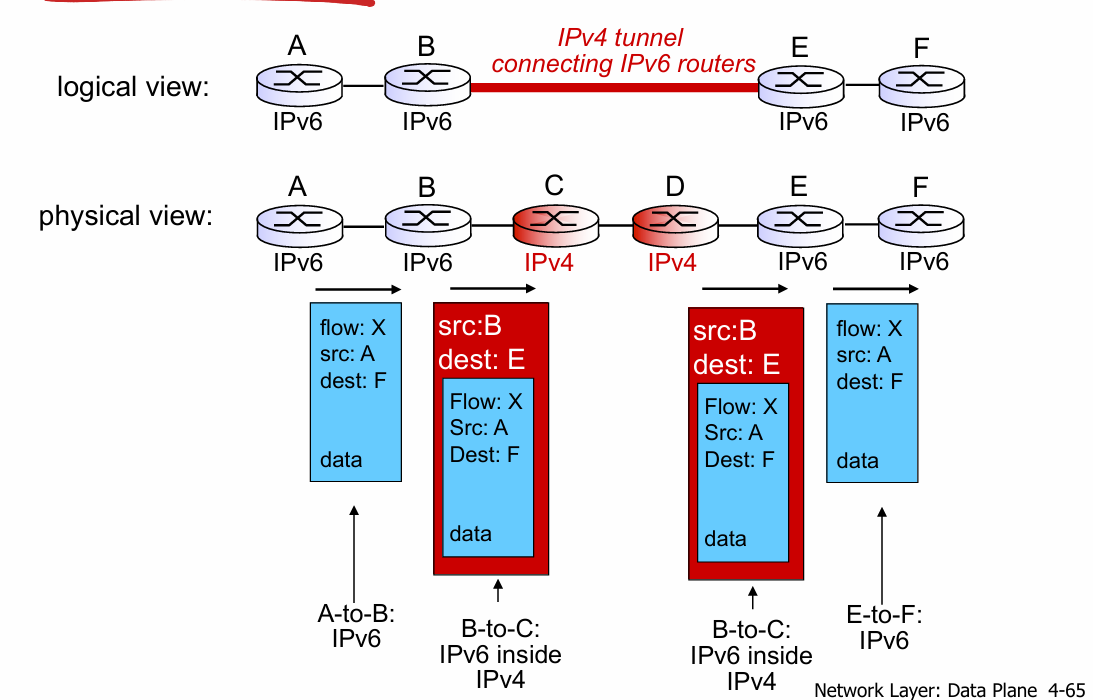
\includegraphics[scale =0.7]{router_28.png}
\caption{%
    \textbf{Tunneling IPv6-in-IPv4.}
    I router B ed E sono \textbf{dual-stack}: hanno due
    interfacce, una IPv6 e una IPv4, con tabelle di
    instradamento ibride (come descritto nella Sezione~3.3.12
    dei tuoi appunti). B incapsula il datagramma IPv6
    in un datagramma IPv4 indirizzato a E (header IPv4
    esterno con src=B, dst=E). I router C e D vedono solo
    un normalissimo datagramma IPv4 e lo inoltrano senza
    sapere cosa contiene. E riconosce che il payload è
    IPv6 , rimuove l'header IPv4 esterno
    e consegna il datagramma IPv6 originale a F.%
}
\label{fig:ipv6-tunneling}
\end{figure}

\begin{notebox}{Adozione di IPv6}
Nonostante sia stato standardizzato nel 1998, l'adozione
di IPv6 è stata molto lenta. Motivi principali: il NAT ha
``risolto'' il problema degli indirizzi nel breve termine
(permettendo a milioni di dispositivi di condividere pochi
IP pubblici); la transizione richiede l'aggiornamento di
tutti i router; nessun singolo attore ha incentivo
sufficiente a fare il primo passo se gli altri non lo fanno.
Tuttavia l'adozione è in accelerazione grazie all'esplosione
dei dispositivi IoT, che rendono insufficiente anche il NAT.
\end{notebox}

\newpage

% ============================================================
\section{Forwarding Generalizzato e SDN}
\label{sec:SDN}
% ============================================================

\subsection{Motivazione: oltre il destination-based forwarding}

Il forwarding tradizionale si basa esclusivamente sull'indirizzo IP di destinazione. Il \textbf{forwarding generalizzato} supera questo limite, permettendo di prendere decisioni di instradamento basate su \textit{qualsiasi} campo dell'header del pacchetto (IP sorgente/destinazione, protocollo, porte TCP/UDP, indirizzi MAC, ecc.).

\subsection{Generalized Forwarding e Flow Tables}

Nell'approccio SDN  (Software-Defined Networking), ogni router contiene una \textbf{flow table} calcolata e distribuita da un controller remoto logicamente centralizzato (come visto nella sezione \ref{:piano controllo}).

\begin{figure}[H]
\centering
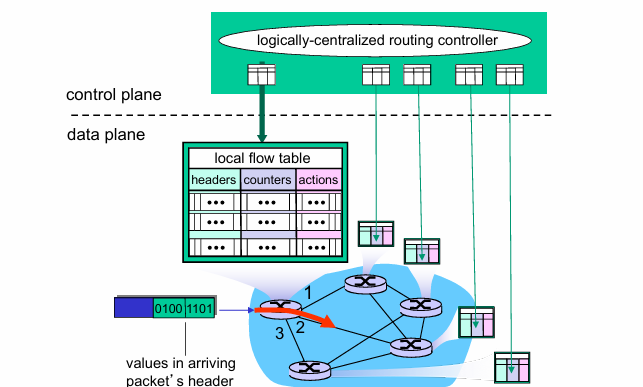
\includegraphics[width=0.75\textwidth]{router_25}
\caption{Architettura SDN. Un controller remoto centralizzato calcola le flow table e le distribuisce a tutti i dispositivi di rete. Ogni router mantiene una copia locale della propria flow table (con i campi match, counters e actions) e la usa per prendere decisioni di forwarding in autonomia, senza dover interrogare il controller per ogni singolo pacchetto.}
\label{fig:sdn-flow-table}
\end{figure}

\newpage

\subsection{OpenFlow: l'astrazione match+action}

\textbf{OpenFlow} è il protocollo standard e più diffuso per la comunicazione tra il controller SDN e i dispositivi di rete. Definisce il formato e il comportamento della flow table.

\begin{defbox}{Astrazione OpenFlow: Match + Action}
Ogni entry (regola) nella flow table OpenFlow è composta da:
\begin{itemize}
    \item \textbf{Pattern (Match)}: valori da confrontare con i campi dell'header del pacchetto in arrivo. Supporta l'uso di wildcard (\texttt{*} = qualsiasi valore).
    \item \textbf{Actions}: l'operazione da eseguire se il pacchetto corrisponde al pattern (es. forward, drop, modify, send-to-controller).
    \item \textbf{Priority}: serve a disambiguare in caso di pattern sovrapposti (vince la regola con la priorità più alta).
    \item \textbf{Counters}: contatori di byte e pacchetti che hanno fatto match con quella regola (fondamentali per le statistiche e il monitoraggio).
\end{itemize}
\end{defbox}

\subsubsection{Campi di match e Azioni in OpenFlow}

Una singola entry OpenFlow può fare match simultaneamente su campi appartenenti a tre livelli differenti dello stack protocollare (Livello Link, Rete e Trasporto):

\begin{figure}[H]
    \centering
    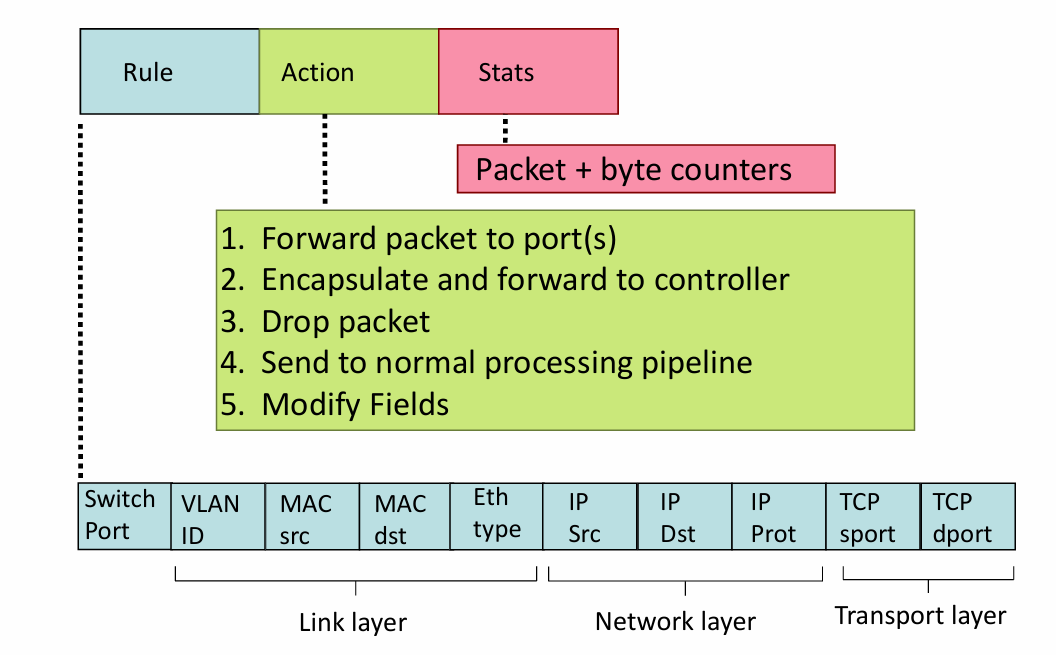
\includegraphics[width=0.6\linewidth]{router_30.png}
    \caption{Campi di match supportati dallo standard OpenFlow.}
    \label{fig:openflow-match}
\end{figure}

Le \textbf{Azioni (Actions)} principali che OpenFlow può applicare sono:
\begin{enumerate}
    \item \textbf{Forward}: inoltra il pacchetto a una o più porte fisiche specifiche.
    \item \textbf{Encapsulate and forward to controller}: incapsula il pacchetto e lo invia al controller SDN (usato tipicamente per pacchetti non riconosciuti).
    \item \textbf{Drop}: scarta il pacchetto silenziosamente.
    \item \textbf{Send to normal processing pipeline}: fa gestire il pacchetto al processo di instradamento tradizionale del router.
    \item \textbf{Modify Fields}: riscrive uno o più campi dell'header prima di inoltrarlo (azione fondamentale per funzioni come il NAT o la QoS).
\end{enumerate}

\subsection{Esempi pratici di regole OpenFlow}

\begin{esempiobox}{Forwarding IP classico (Comportamento da Router)}
Invia tutti i datagrammi destinati all'IP \texttt{51.6.0.8} alla porta di uscita 6.
\begin{center}
\resizebox{\textwidth}{!}{
\begin{tabular}{lllllllllll}
\toprule
\textbf{Port} & \textbf{MAC src} & \textbf{MAC dst} & \textbf{EthType} & \textbf{VLAN} & \textbf{IP src} & \textbf{IP dst} & \textbf{IP prot} & \textbf{TCP sport} & \textbf{TCP dport} & \textbf{Action} \\
\midrule
* & * & * & * & * & * & 51.6.0.8 & * & * & * & \textbf{port6} \\
\bottomrule
\end{tabular}
}
\end{center}
\end{esempiobox}

\begin{esempiobox}{Firewall - Blocco per porta}
Scarta tutti i datagrammi destinati alla porta TCP 22 (Blocca il traffico SSH).
\begin{center}
\resizebox{\textwidth}{!}{
\begin{tabular}{lllllllllll}
\toprule
\textbf{Port} & \textbf{MAC src} & \textbf{MAC dst} & \textbf{EthType} & \textbf{VLAN} & \textbf{IP src} & \textbf{IP dst} & \textbf{IP prot} & \textbf{TCP sport} & \textbf{TCP dport} & \textbf{Action} \\
\midrule
* & * & * & * & * & * & * & * & * & 22 & \textbf{drop} \\
\bottomrule
\end{tabular}
}
\end{center}
\end{esempiobox}

\begin{esempiobox}{Firewall - Blocco per IP sorgente}
Scarta tutti i datagrammi inviati dall'host \texttt{128.119.1.1}.
\begin{center}
\resizebox{\textwidth}{!}{
\begin{tabular}{lllllllllll}
\toprule
\textbf{Port} & \textbf{MAC src} & \textbf{MAC dst} & \textbf{EthType} & \textbf{VLAN} & \textbf{IP src} & \textbf{IP dst} & \textbf{IP prot} & \textbf{TCP sport} & \textbf{TCP dport} & \textbf{Action} \\
\midrule
* & * & * & * & * & 128.119.1.1 & * & * & * & * & \textbf{drop} \\
\bottomrule
\end{tabular}
}
\end{center}
\end{esempiobox}

\begin{esempiobox}{Layer 2 forwarding (Comportamento da Switch)}
Inoltra i frame Ethernet provenienti dal MAC \texttt{22:A7:23:11:E1:02} alla porta 3.
\begin{center}
\resizebox{\textwidth}{!}{
\begin{tabular}{lllllllllll}
\toprule
\textbf{Port} & \textbf{MAC src} & \textbf{MAC dst} & \textbf{EthType} & \textbf{VLAN} & \textbf{IP src} & \textbf{IP dst} & \textbf{IP prot} & \textbf{TCP sport} & \textbf{TCP dport} & \textbf{Action} \\
\midrule
* & 22:A7:23... & * & * & * & * & * & * & * & * & \textbf{port3} \\
\bottomrule
\end{tabular}
}
\end{center}
\end{esempiobox}


\subsection{Esempio completo: rete OpenFlow con instradamento generalizzato}

\begin{figure}[H]
\centering
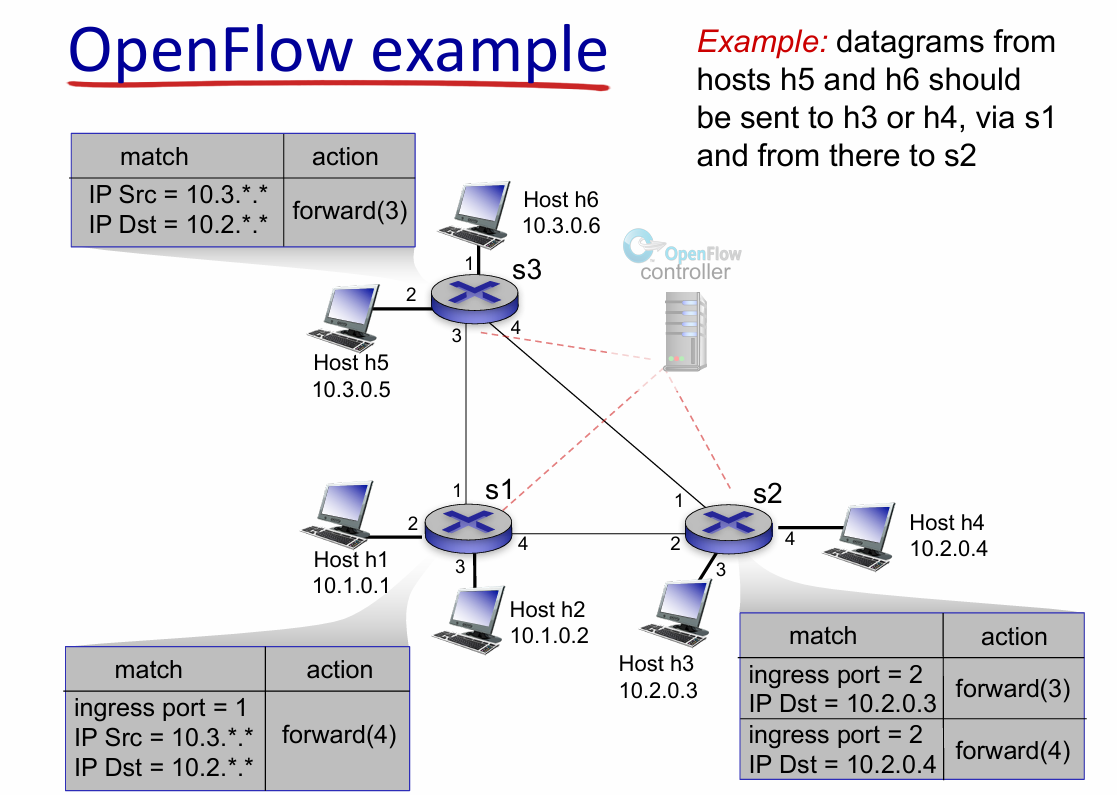
\includegraphics[width=0.85\textwidth]{router_31}
\caption{%
    \textbf{Esempio di routing basato sulla sorgente tramite dispositivi OpenFlow.} 
    La rete mostra tre nodi OpenFlow ($s1, s2, s3$) e sei host ($h1$--$h6$). In questo scenario, il controller SDN ha programmato le \textit{flow table} per superare i limiti del forwarding tradizionale: il traffico proveniente dall'IP di \textbf{h5} viene instradato verso la destinazione seguendo il percorso \texttt{s3 $\to$ s1 $\to$ s2}, mentre il traffico di \textbf{h6} (stessa destinazione) segue un percorso differente. Questo è possibile perché i dispositivi, pur agendo come router di livello 3, possono differenziare il percorso in base all'IP sorgente o ad altri parametri di match.
}
\label{fig:openflow-example}
\end{figure}

\begin{collegamentobox}[title=�� Collegamento Inter-Capitolo: SDN unifica i dispositivi di rete]
La vera potenza del paradigma \textbf{Match + Action} di OpenFlow è la capacità di trasformare un singolo dispositivo programmabile in uno qualsiasi degli apparati studiati nei capitoli precedenti, eliminando la distinzione hardware tra switch e router:
\begin{itemize}
    \item \textbf{Router (Cap. 5)}: match sul prefisso IP di destinazione e azione \texttt{forward}.
    \item \textbf{Switch L2 (Cap. 3)}: match sul MAC address di destinazione e azione \texttt{forward}.
    \item \textbf{Firewall Stateless (Cap. 4)}: match su IP/porta e azione \texttt{drop}.
    \item \textbf{NAT (Cap. 3)}: match su IP+porta e azione \texttt{modify fields} (riscrittura indirizzi).
\end{itemize}
Un controller SDN centralizzato può quindi "decidere" la personalità del dispositivo semplicemente aggiornando le righe della sua flow table.
\end{collegamentobox}

% ============================================================
\section{Riepilogo del Piano dei Dati}
% ============================================================

\begin{tcolorbox}[colback=unibolight, colframe=uniboblue, title=\bfseries Concetti chiave del Capitolo 5 (Data Plane), breakable]

\textit{Nota: Gli argomenti logici (DHCP, NAT, CIDR, Subnetting) sono stati trasferiti  Capitolo 3. Questo capitolo si concentra sull'hardware e la fisica dei router.}

\begin{enumerate}
    \item \textbf{Data Plane vs Control Plane}: Il \textit{Data Plane} opera in hardware locale su ogni singolo router (forwarding rapidissimo in nanosecondi); il \textit{Control Plane} opera via software, calcolando i percorsi globali dell'intera rete (routing in millisecondi).
    
    \item \textbf{Architettura fisica del router}: È composto da \textit{porte di ingresso} (ricezione, code e lookup), una \textit{switching fabric} (basata su memoria, bus o crossbar per spostare fisicamente i pacchetti), \textit{porte di uscita} (code e scheduling) e un \textit{routing processor}.
    
    \item \textbf{Longest Prefix Matching (LPM)}: È la regola aurea del forwarding IP. Tra più regole coincidenti, il router instradato usa sempre quella con il prefisso di rete più specifico (la maschera più lunga). L'LPM è eseguito a velocità hardware tramite memorie speciali chiamate \textbf{TCAM}.
    
    \item \textbf{Code e HOL Blocking}: Nelle porte di ingresso, un pacchetto fermo in testa alla coda impedisce l'avanzamento dei pacchetti dietro di lui, anche se questi ultimi devono raggiungere porte di uscita completamente libere (\textit{Head-Of-Line Blocking}).
    
    \item \textbf{Buffer di Uscita e TCP (Collegamento Logico)}: Nelle porte di uscita, quando i pacchetti arrivano più velocemente di quanto il link riesca a smaltirli, il buffer si satura e scarta le nuove connessioni (\textit{Tail Drop}). \textbf{È questo scarto fisico} che innesca la perdita rilevata dal TCP, portandolo al \textit{Timeout} e al dimezzamento della \textit{Sliding Window} (Capitolo 3).
    
    \item \textbf{Scheduling e Qualità del Servizio (QoS)}: Il Ritardo di Accodamento e il Jitter nascono dentro i router. Per garantire la fluidità (es. al VoIP), i router smistano le code di uscita usando algoritmi come \textbf{FIFO}, \textbf{Priority Queuing} (passano prima i VIP) e \textbf{WFQ (Weighted Fair Queuing)} (che divide proporzionalmente la banda evitando la \textit{starvation} delle code meno importanti).
    
    \item \textbf{Il Datagramma IPv4}: Ha un overhead obbligatorio di \textbf{20 byte} per ogni pacchetto. Oltre agli IP, l'header include il \textit{TTL} (per uccidere i pacchetti in loop), il \textit{Checksum} e l'indicatore del protocollo superiore (TCP/UDP).
    
    \item \textbf{Frammentazione}: Se un datagramma è più grande della MTU del cavo su cui deve transitare, il router usa i campi dell'header IPv4 (\textit{Identifier}, \textit{Flags} e \textit{Offset}) per dividerlo in pacchetti più piccoli. Essi verranno riassemblati solo dal computer di destinazione finale, mai dai router intermedi.

    \item \textbf{Il Datagramma IPv6}: progettato per l'efficienza hardware con indirizzi a 128 bit  e un header a lunghezza fissa di \textbf{40 byte}. A differenza di IPv4, rimuove il checksum dell'header e la frammentazione nei router intermedi per velocizzare l'inoltro.
    
    \item \textbf{SDN e OpenFlow}: Il \textit{Forwarding Generalizzato} (SDN) sposta l'intelligenza su un controller remoto. Con il paradigma \textbf{Match + Action} delle flow tables (OpenFlow), un singolo dispositivo di rete programmabile può emulare contemporaneamente un Router, uno Switch, un Firewall o un NAT.
\end{enumerate}

\vspace{0.3cm}
\textbf{Domanda aperta per il prossimo modulo}: Abbiamo visto come l'hardware muove i pacchetti seguendo le tabelle, ma \textit{come vengono calcolate matematicamente a monte queste tabelle dai router}? $\Rightarrow$ Lo scopriremo nel prossimo capitolo analizzando il \textbf{Piano di Controllo  CAP 6 (Routing e Algoritmi)}.
\end{tcolorbox}



\end{document}
